\documentclass[journal,compsoc, 10pt, draftclsnofoot, onecolumn]{IEEEtran}

\usepackage{graphicx}
\usepackage{amssymb}
\usepackage{amsmath}
\usepackage{amsthm}
\usepackage{tabularx}
\usepackage{graphicx}

\newcommand{\subparagraph}{}
\usepackage{titlesec}

\usepackage{alltt}
\usepackage{float}
\usepackage{color}
\usepackage{url}

\usepackage{balance}
\usepackage[TABBOTCAP, tight]{subfigure}
\usepackage{enumitem}
\usepackage{pstricks, pst-node}

\usepackage{cite}
\usepackage{listings}
\usepackage{placeins}

\usepackage[margin=0.75in]{geometry}
\geometry{textheight=8.5in, textwidth=6in}

\renewcommand{\familydefault}{\sfdefault}

\newlength\tindent
\setlength{\tindent}{\parindent}
\setlength{\parindent}{0pt}
\renewcommand{\indent}{\hspace*{\tindent}}

\newcommand{\cred}[1]{{\color{red}#1}}
\newcommand{\cblue}[1]{{\color{blue}#1}}

\newcommand{\namesigdate}[2][6cm]{%
  \begin{tabular}{@{}p{#1}@{}}
    #2 \\[0.5\normalbaselineskip] \hrule \\[0.pt]
    {\small \vspace{-3em} \textit{Signature}} \\[0.5\normalbaselineskip] \hrule \\[0pt]
    {\small \vspace{-3em}\textit{Date}}
  \end{tabular}
}


\usepackage{hyperref}
\usepackage{geometry}

\lstset{
language=C,
basicstyle=\ttfamily,
commentstyle=\color{blue},
numberstyle=\color{red},
stringstyle=\color{orange}
}

\def\nameD{Devin Foulger}
\def\nameH{Hector Trujillo}
\def\nameB{Bryan Liauw}

\usepackage{fancyvrb}
\usepackage{color}
\usepackage[latin1]{inputenc}


\makeatletter
\def\PY@reset{\let\PY@it=\relax \let\PY@bf=\relax%
    \let\PY@ul=\relax \let\PY@tc=\relax%
    \let\PY@bc=\relax \let\PY@ff=\relax}
\def\PY@tok#1{\csname PY@tok@#1\endcsname}
\def\PY@toks#1+{\ifx\relax#1\empty\else%
    \PY@tok{#1}\expandafter\PY@toks\fi}
\def\PY@do#1{\PY@bc{\PY@tc{\PY@ul{%
    \PY@it{\PY@bf{\PY@ff{#1}}}}}}}
\def\PY#1#2{\PY@reset\PY@toks#1+\relax+\PY@do{#2}}

\expandafter\def\csname PY@tok@gd\endcsname{\def\PY@tc##1{\textcolor[rgb]{0.63,0.00,0.00}{##1}}}
\expandafter\def\csname PY@tok@gu\endcsname{\let\PY@bf=\textbf\def\PY@tc##1{\textcolor[rgb]{0.50,0.00,0.50}{##1}}}
\expandafter\def\csname PY@tok@gt\endcsname{\def\PY@tc##1{\textcolor[rgb]{0.00,0.25,0.82}{##1}}}
\expandafter\def\csname PY@tok@gs\endcsname{\let\PY@bf=\textbf}
\expandafter\def\csname PY@tok@gr\endcsname{\def\PY@tc##1{\textcolor[rgb]{1.00,0.00,0.00}{##1}}}
\expandafter\def\csname PY@tok@cm\endcsname{\let\PY@it=\textit\def\PY@tc##1{\textcolor[rgb]{0.25,0.50,0.50}{##1}}}
\expandafter\def\csname PY@tok@vg\endcsname{\def\PY@tc##1{\textcolor[rgb]{0.10,0.09,0.49}{##1}}}
\expandafter\def\csname PY@tok@m\endcsname{\def\PY@tc##1{\textcolor[rgb]{0.40,0.40,0.40}{##1}}}
\expandafter\def\csname PY@tok@mh\endcsname{\def\PY@tc##1{\textcolor[rgb]{0.40,0.40,0.40}{##1}}}
\expandafter\def\csname PY@tok@go\endcsname{\def\PY@tc##1{\textcolor[rgb]{0.50,0.50,0.50}{##1}}}
\expandafter\def\csname PY@tok@ge\endcsname{\let\PY@it=\textit}
\expandafter\def\csname PY@tok@vc\endcsname{\def\PY@tc##1{\textcolor[rgb]{0.10,0.09,0.49}{##1}}}
\expandafter\def\csname PY@tok@il\endcsname{\def\PY@tc##1{\textcolor[rgb]{0.40,0.40,0.40}{##1}}}
\expandafter\def\csname PY@tok@cs\endcsname{\let\PY@it=\textit\def\PY@tc##1{\textcolor[rgb]{0.25,0.50,0.50}{##1}}}
\expandafter\def\csname PY@tok@cp\endcsname{\def\PY@tc##1{\textcolor[rgb]{0.74,0.48,0.00}{##1}}}
\expandafter\def\csname PY@tok@gi\endcsname{\def\PY@tc##1{\textcolor[rgb]{0.00,0.63,0.00}{##1}}}
\expandafter\def\csname PY@tok@gh\endcsname{\let\PY@bf=\textbf\def\PY@tc##1{\textcolor[rgb]{0.00,0.00,0.50}{##1}}}
\expandafter\def\csname PY@tok@ni\endcsname{\let\PY@bf=\textbf\def\PY@tc##1{\textcolor[rgb]{0.60,0.60,0.60}{##1}}}
\expandafter\def\csname PY@tok@nl\endcsname{\def\PY@tc##1{\textcolor[rgb]{0.63,0.63,0.00}{##1}}}
\expandafter\def\csname PY@tok@nn\endcsname{\let\PY@bf=\textbf\def\PY@tc##1{\textcolor[rgb]{0.00,0.00,1.00}{##1}}}
\expandafter\def\csname PY@tok@no\endcsname{\def\PY@tc##1{\textcolor[rgb]{0.53,0.00,0.00}{##1}}}
\expandafter\def\csname PY@tok@na\endcsname{\def\PY@tc##1{\textcolor[rgb]{0.49,0.56,0.16}{##1}}}
\expandafter\def\csname PY@tok@nb\endcsname{\def\PY@tc##1{\textcolor[rgb]{0.00,0.50,0.00}{##1}}}
\expandafter\def\csname PY@tok@nc\endcsname{\let\PY@bf=\textbf\def\PY@tc##1{\textcolor[rgb]{0.00,0.00,1.00}{##1}}}
\expandafter\def\csname PY@tok@nd\endcsname{\def\PY@tc##1{\textcolor[rgb]{0.67,0.13,1.00}{##1}}}
\expandafter\def\csname PY@tok@ne\endcsname{\let\PY@bf=\textbf\def\PY@tc##1{\textcolor[rgb]{0.82,0.25,0.23}{##1}}}
\expandafter\def\csname PY@tok@nf\endcsname{\def\PY@tc##1{\textcolor[rgb]{0.00,0.00,1.00}{##1}}}
\expandafter\def\csname PY@tok@si\endcsname{\let\PY@bf=\textbf\def\PY@tc##1{\textcolor[rgb]{0.73,0.40,0.53}{##1}}}
\expandafter\def\csname PY@tok@s2\endcsname{\def\PY@tc##1{\textcolor[rgb]{0.73,0.13,0.13}{##1}}}
\expandafter\def\csname PY@tok@vi\endcsname{\def\PY@tc##1{\textcolor[rgb]{0.10,0.09,0.49}{##1}}}
\expandafter\def\csname PY@tok@nt\endcsname{\let\PY@bf=\textbf\def\PY@tc##1{\textcolor[rgb]{0.00,0.50,0.00}{##1}}}
\expandafter\def\csname PY@tok@nv\endcsname{\def\PY@tc##1{\textcolor[rgb]{0.10,0.09,0.49}{##1}}}
\expandafter\def\csname PY@tok@s1\endcsname{\def\PY@tc##1{\textcolor[rgb]{0.73,0.13,0.13}{##1}}}
\expandafter\def\csname PY@tok@sh\endcsname{\def\PY@tc##1{\textcolor[rgb]{0.73,0.13,0.13}{##1}}}
\expandafter\def\csname PY@tok@sc\endcsname{\def\PY@tc##1{\textcolor[rgb]{0.73,0.13,0.13}{##1}}}
\expandafter\def\csname PY@tok@sx\endcsname{\def\PY@tc##1{\textcolor[rgb]{0.00,0.50,0.00}{##1}}}
\expandafter\def\csname PY@tok@bp\endcsname{\def\PY@tc##1{\textcolor[rgb]{0.00,0.50,0.00}{##1}}}
\expandafter\def\csname PY@tok@c1\endcsname{\let\PY@it=\textit\def\PY@tc##1{\textcolor[rgb]{0.25,0.50,0.50}{##1}}}
\expandafter\def\csname PY@tok@kc\endcsname{\let\PY@bf=\textbf\def\PY@tc##1{\textcolor[rgb]{0.00,0.50,0.00}{##1}}}
\expandafter\def\csname PY@tok@c\endcsname{\let\PY@it=\textit\def\PY@tc##1{\textcolor[rgb]{0.25,0.50,0.50}{##1}}}
\expandafter\def\csname PY@tok@mf\endcsname{\def\PY@tc##1{\textcolor[rgb]{0.40,0.40,0.40}{##1}}}
\expandafter\def\csname PY@tok@err\endcsname{\def\PY@bc##1{\setlength{\fboxsep}{0pt}\fcolorbox[rgb]{1.00,0.00,0.00}{1,1,1}{\strut ##1}}}
\expandafter\def\csname PY@tok@kd\endcsname{\let\PY@bf=\textbf\def\PY@tc##1{\textcolor[rgb]{0.00,0.50,0.00}{##1}}}
\expandafter\def\csname PY@tok@ss\endcsname{\def\PY@tc##1{\textcolor[rgb]{0.10,0.09,0.49}{##1}}}
\expandafter\def\csname PY@tok@sr\endcsname{\def\PY@tc##1{\textcolor[rgb]{0.73,0.40,0.53}{##1}}}
\expandafter\def\csname PY@tok@mo\endcsname{\def\PY@tc##1{\textcolor[rgb]{0.40,0.40,0.40}{##1}}}
\expandafter\def\csname PY@tok@kn\endcsname{\let\PY@bf=\textbf\def\PY@tc##1{\textcolor[rgb]{0.00,0.50,0.00}{##1}}}
\expandafter\def\csname PY@tok@mi\endcsname{\def\PY@tc##1{\textcolor[rgb]{0.40,0.40,0.40}{##1}}}
\expandafter\def\csname PY@tok@gp\endcsname{\let\PY@bf=\textbf\def\PY@tc##1{\textcolor[rgb]{0.00,0.00,0.50}{##1}}}
\expandafter\def\csname PY@tok@o\endcsname{\def\PY@tc##1{\textcolor[rgb]{0.40,0.40,0.40}{##1}}}
\expandafter\def\csname PY@tok@kr\endcsname{\let\PY@bf=\textbf\def\PY@tc##1{\textcolor[rgb]{0.00,0.50,0.00}{##1}}}
\expandafter\def\csname PY@tok@s\endcsname{\def\PY@tc##1{\textcolor[rgb]{0.73,0.13,0.13}{##1}}}
\expandafter\def\csname PY@tok@kp\endcsname{\def\PY@tc##1{\textcolor[rgb]{0.00,0.50,0.00}{##1}}}
\expandafter\def\csname PY@tok@w\endcsname{\def\PY@tc##1{\textcolor[rgb]{0.73,0.73,0.73}{##1}}}
\expandafter\def\csname PY@tok@kt\endcsname{\def\PY@tc##1{\textcolor[rgb]{0.69,0.00,0.25}{##1}}}
\expandafter\def\csname PY@tok@ow\endcsname{\let\PY@bf=\textbf\def\PY@tc##1{\textcolor[rgb]{0.67,0.13,1.00}{##1}}}
\expandafter\def\csname PY@tok@sb\endcsname{\def\PY@tc##1{\textcolor[rgb]{0.73,0.13,0.13}{##1}}}
\expandafter\def\csname PY@tok@k\endcsname{\let\PY@bf=\textbf\def\PY@tc##1{\textcolor[rgb]{0.00,0.50,0.00}{##1}}}
\expandafter\def\csname PY@tok@se\endcsname{\let\PY@bf=\textbf\def\PY@tc##1{\textcolor[rgb]{0.73,0.40,0.13}{##1}}}
\expandafter\def\csname PY@tok@sd\endcsname{\let\PY@it=\textit\def\PY@tc##1{\textcolor[rgb]{0.73,0.13,0.13}{##1}}}

\def\PYZbs{\char`\\}
\def\PYZus{\char`\_}
\def\PYZob{\char`\{}
\def\PYZcb{\char`\}}
\def\PYZca{\char`\^}
\def\PYZam{\char`\&}
\def\PYZlt{\char`\<}
\def\PYZgt{\char`\>}
\def\PYZsh{\char`\#}
\def\PYZpc{\char`\%}
\def\PYZdl{\char`\$}
\def\PYZti{\char`\~}
% for compatibility with earlier versions
\def\PYZat{@}
\def\PYZlb{[}
\def\PYZrb{]}
\makeatother


\hypersetup {
        colorlinks = true,
        urlcolor = black,
        linkcolor = black,
        pdfauthor = {\nameD\nameH\nameB},
        pdfkeywords = {},
        pdfsubject = {},
        pdfpagemode = UseNone
}

\titleformat{\section}
	{\normalfont\fontsize{15}{10}\bfseries}{\thesection}{1em}{}
\titleformat{\subsection}
	{\normalfont\fontsize{12}{15}\bfseries}{\thesubsection}{1em}{}
\titleformat{\subsubsection}
	{\normalfont\fontsize{12}{15}\bfseries}{\thesubsubsection}{1em}{}

\begin{document}

\title{\vspace{20em}Final Documentation \\{\vspace{-1ex}\huge UniversityGear} \\ {\large
\today \\ CS463 Spring Term}}
\author{\vspace{10ex}Devin Foulger \\{\vspace{-1ex}Hector Trujillo} \\{\vspace{-1ex}Bryan
Liauw}}

\begin{titlepage}

\maketitle
\thispagestyle{empty}

\begin{figure}[!h]

\centering

\includegraphics[scale=.6]{ugear_launcher}
\end{figure}
\FloatBarrier

\begin{abstract}
This document will recap what we have done over the term and will describe what we plan to do
in the following year. It will go
into detail about the goals we have set and how we plan to accomplish them. It will also
include a summary of the project status as it
is now. It will also include a retrospective of what has happened throughout the term.
\end{abstract}

\end{titlepage}

\tableofcontents

\section{Introduction}
UniversityGear is an application that allows for any to browse for college and 
university related merchandise. This could be anything from textbooks to sports 
gear. This project was requested by eBay, where Luther Boorn acted as the client. 
The importance of this project was to design an Android application using eBay's 
new public APIs. The application will be used to help demonstrate how to use 
eBay's APIs for people who want to build targeted eBay experiences. \newline

There are three members to the UniversityGear team: Devin Foulger, Hector 
Trujillo, and Bryan Liauw. Devin's role in the group was to create backend 
classes as well as work on user interface design. Hector focused mostly on 
the user interface and Bryan worked on the backend of the application. 
However, all of the group members helped each other and worked on 
all aspects of the application. With the help from Luther and the other mentor's 
at eBay, we were able to successfully create our application. 

\section{Requirements}

\subsection{Introduction}

This section will provide an overview of what is included in this Software 
Requirements Document (SRS).

\subsubsection{Purpose}

This SRS document will serve several purposes. First it will define the 
requirements for the "UniversityGear" application that team "4Credit"
 will be developing for their CS Capstone project for eBay. The 
document will be detailing the constraints, features, dependencies and performance 
of the application in a manner that clearly demonstrates what the client will be
 receiving.The intended audience for this Software Requirements Specification 
(SRS) will be the team, eBay, and the instructors of the computer science senior
 capstone class at Oregon State University. 

\subsubsection{Scope}

The Android Application, "UniversityGear", will allow users to browse and 
shop for college merchandise that are for sale through eBay. The application 
will be published to the Google Play Store and will be optimized for Android's 
latest operating system 'N'. \newline

This application will also demonstrate the use and functionality of eBay's 
public APIs by allowing users to search eBay's inventory of items. The 
application will allow users to filter out their search results by different 
criteria. The application will also allow users to purchase items from eBay. 

\subsubsection{Definitions, acronyms, and abbreviations}

Below are definitions for terms that will allow for proper interpretation of the
 requirements document.

\begin{table}[!h]
\centering
\caption{Definitions}
\label{Definition table}
\begin{tabularx}{\textwidth}{l|X}
\hline
\textbf{Term}               & \textbf{Definition}   \\ \hline
API                    	      & Application Programming Interface, allows developers to
 develop applications that connect to eBay's large inventory of items. \\ \hline
Shop                   	      & Search for and view college related items on sale 
through eBay. \\ \hline
Vendors               	      & Individuals or companies that sell or will sell items on 
eBay\\ \hline
Filters                	      & Search criteria that will allow the user to more easily 
find the item that they are looking for. \\ \hline
Third-Party Developers & Individuals outside of eBay that will be using eBay's public 
APIs to create their own applications.\\ \hline
Application            	      & An Android application that uses eBay's public 
APIs. \\ \hline
Interface              	      & The User Interface.\\ \hline
College Merchandise     & Items such as school supplies for Higher Ed, fan gear, 
etc...   \\ \hline
User                   	      & Any one who will be using the Android Application 
utilizing eBay's APIs.\\ \hline
Client                 	      & eBay  \\ \hline
BIN                    	      & Buy It Now      \\ \hline
N                   	      & Android's new Nougat operating system 
\\ \hline
M                   	      & Android's Marshmallow operating system\\ \hline
\end{tabularx}
\end{table}

\newpage

\subsubsection{Overview}

The remainder of this document will provide an overview of the functionality 
that the "UniversityGear" application will offer along with the 
interaction that it will have with other systems. The next chapter will identify
 any constraints that may prevent success for this project.

\subsection{Overall Description}

This section will provide the reader with an overview of the entire application.
 The application will be explained in a way that the functionality is easily 
identified along with any constraints.

\subsubsection{Product Perspective}

The android application will communicate with eBay to provide the user with the 
opportunity to shop through their inventory of college related merchandise. The 
communication will be accomplished with the use of eBay's APIs. This 
communication is important to provide the user with a seamless shopping 
experience without having to switch between different applications.\newline

Since no data regarding the inventory of items that eBay provides will be stored
 by this application, there will be a constant need for an Internet connection 
to be able to pull search results from eBay's inventory. 

\subsubsection{User Interfaces}

The user interface will mimic what people already know about eBay and other 
similar shopping experiences. This will include standard things such as a place 
to search for items, and a place to view items. Searching 
could also vary depending on search settings like a basic search or advanced 
searching. When viewing items, there could be several kinds of list views. We 
would also have specific college-related images to help users to find the item 
that they are looking for. Since our application is limited to college 
merchandises, we will have some visual appeals that reflect what the application
 is about.

\subsubsection{Hardware Interfaces}

The devices that we use must be compatible with M and N os. 

\subsubsection{Software Interfaces}

We will be using the new Android operating system, N. We will also be making use
 of a wide variety of eBay's new APIs. Some of these are apart of their new Buy 
APIs. These ones include the Browse and Order APIs. The Browse API will allow us
 to search for items and find different item feeds. The Order API will allow us 
to have some form of item checkout and order tracking. Together, these APIs
 will allow us to connect with eBay's large collection of items. We also plan 
on using their Guest Checkout API, so that users will be able to purchase items.

\subsubsection{Communication Interfaces}

The device should always have some form of connection to the internet. This 
means the device can connect in one of two ways. The first being through the 
devices WLAN. The second being that it could connect using its cellular data.

\subsubsection{Operations}

There will be many user initiated operations. These include searching and 
purchasing. Searching means that the user will be finding items with specific 
search criteria. The items that they find could be related to different schools,
 or have specific colors. Purchasing means that the user is able to select an 
item that they want and pay for it.\newline

The application should only be in use when a user is actually using it. There 
are no periods of unattended use. The only time that might be considered as 
unattended use, is when the application is gathering and displaying search 
results to the user. 

\subsubsection{Production Functions}

There are a couple of major features that this application will support. It will
 allow for users to search for items and to purchase them. Users will be able 
to browse eBay's large collection of college merchandise that they have for 
sale. The application will allow users to narrow down what they are looking for 
by allowing them to use filters such as types of items, condition, cost, college
 specific, by terms, and so on. \newline

The results of these searches will be displayed in either a listview that simply
 provides minor details regarding the item or thumbnail views that provide an 
image of the product along with a few details. The number of results displayed 
at once will vary depending on how the user wants the results presented to them 
and by the screen size of the product that they will be using. The application 
will also allow the user to sort the order in which the items are displayed. The
 sort options will be similar to what eBay provides on their current website. 
This includes sorting by price or condition.

\subsubsection{User Characteristics}

Users will include individuals who are looking to find great deals on college 
merchandise online. The typical user will be someone who is looking for college 
merchandise. The actual user group could range between many different people. 
The main audience should be individuals looking for college merchandise and 
could be incoming college students, or people who are already college students. 
Users could also be parents, grandparents or other individuals who are looking 
to help out a relative or friend in searching for any college merchandise that 
the individual might need. \newline

Since are users are going to use this application on  a mobile device, 
our main focus to the user would be to create an interface that is simple
 and straightforward. The user should be able to learn and familiarize with the interface
 in a short period of time. Furthermore, the processes should be fast; the 
window between processes should be short to keep the attention of the users.

\subsubsection{Constraints}

Android's new operating system, N OS, will be the biggest constraint. This is 
because the operating system is new and is not present on many of today's top 
Android devices. This also means that the documentation may not be up to date 
with the new operating system. Older APIs created by Google may also be
 deprecated.\newline

Large loads on the application might put strain on lower quality machines. 
Example of large loads would be a lot of activities and threads and overly 
large image.Testing might also be a constraint since a virtual machine will take a huge 
amount of computer resources. For a better testing environment, the usage of an 
actual physical smartphone might be needed.

\subsubsection{Assumptions and Dependancies}

An assumption and dependency for this project will be the availability of the 
Android operating system N and a device that can run it. A secondary assumption 
is that the mobile phone which the application will be running on will have an 
active internet connection. A third assumption would be that users of the 
application will have an eBay account that they will be able to use to save 
searched items and even checkout and complete a purchase through the 
application. A dependency that the application will have is that we highly 
depends on the connection to the eBay database. If the database server is down, 
we might not get the app to work.

\subsection{Specific Requirements}

\subsubsection{Functional Requirements}

This section defines all the requirements that are fundamental actions to the 
application.

\subsubsection*{Functional Requirement 1}
Name: Download application \newline
Description: The user must be able to download the application from the Google 
Play store. \newline
Input: None. \newline
Output: Application will be installed on the user's device. \newline
Dependencies: The user has an Android device that can support N os.

\subsubsection*{Functional Requirement 2}
Name: Update application\newline
Description: This should allow the user to update the application via the Google
 Play store.\newline
Input: None.\newline
Output: Update application.\newline
Dependencies: The user has an Android device that can support N os.

\subsubsection*{Functional Requirement 3}
Name: Determine search criteria\newline
Description: The user should be able to select what they want to search for. The
 user should be able to select between many options. These include search by BIN
 (Buy It Now), price, school, color, and condition. They should also be
 able to use different search criteria in combination.\newline
Input: A combination of the above stated search criteria.\newline
Output: None.\newline
Dependencies: Functional requirement 1.

\subsubsection*{Functional Requirement 4}
Name: Guest Checkout\newline
Description: The user should be able to purchase an item that they have searched
 for.\newline
Input: The item that is going to be purchased.\newline
Output: Some receipt or confirmation that the item has been ordered.\newline
Dependencies: Functional requirement 4.

\subsubsection*{Functional Requirement 5}
Name: Display search results\newline
Description: Search results should be displayed to the user given the user's 
search criteria. Search results should also be displayed according to how the 
user specifies. That should be able to display results from lowest price to 
largest price, or from BIN to bid.\newline
Input: None.\newline
Output: A list of items organized the way the user has specified.\newline
Dependencies: Functional requirements 4.

\subsubsection*{Functional Requirement 6}
Name: Display search results (no results found)\newline
Description: This should display a list that doesn't include any items and will 
have a simple message stating that no items could be found. \newline
Input: None.\newline
Output: A simple message that states nothing could be found.\newline
Dependencies: Functional requirement 4.

\subsubsection*{Functional Requirement 7}
Name: Item view for a selected item\newline
Description: When a user selects an item, it should be displayed in its own view
 with greater detail.\newline
Input: Item from listview.\newline
Output: A page with complete detail of the item.\newline
Dependencies: Functional requirement 10.

\subsubsection*{Functional Requirement 8}
Name: Save search criteria\newline
Description: The user should be able to fill out and pick specific search terms
that will be saved for later use. For example, someone who searches for Oregon 
State University gear with the color orange, will be able to save that information
for later use.\newline
Input: User specified search criteria.\newline
Output: A saved search filter.\newline
Dependencies: Functional requirement 

\subsubsection{Stretch Goals}

This section will define any stretch goals.

\subsubsection*{Stretch Goal 1}
Name: Shopping Cart\newline
Description: This is where items would be saved before users want to
purchase the items. A user should be able to view their shopping cart with
the items they have selected.\newline
Input: Items they have selected.\newline
Output: A page with the items they want to purchase.\newline
Dependencies: Functional requirement 4.

\subsubsection{Performance Requirements}

This section will document that the requirements provide a measurement of how 
the application will perform.

\subsubsection*{Performance Requirement 1}
Name: Search feature\newline
Measurement: The search feature should be easy to find and easy to use.\newline
Dependencies: None.

\subsubsection*{Performance Requirement 2}
Name: Usage of search feature\newline
Measurement: The search criteria provided should be easy to understand and 
simple.\newline
Dependencies: Performance requirement 1.

\subsubsection*{Performance Requirement 3}
Name: Usage of search results in a listview\newline
Measurement: The results displayed in a listview should provide the user with 
easy to understand results. Things like the item name, price, and school should 
be provided to the user.\newline
Dependencies: Performance requirement 1.

\subsubsection*{Performance Requirement 4}
Name: Usage of purchase feature\newline
Measurement: Users should receive a receipt that the feature worked. Users 
should also be notified that the payment is being processed, as PayPal can
be slow at times.\newline 
Dependencies: Performance requirement 4.

\subsubsection*{Performance Requirement 5}
Name: Connectivity \newline
Measurement: If no internet connection is present, the application will inform
the user that they need a connection to continue using the app.
Dependencies: None.

\subsubsection{Software System Attributes}

This section will define how are application will meet the software system 
attributes.

\subsubsection*{Reliability}

The application should be able to search and purchase items according to what 
has been specified by the user. We also make sure that our application will 
have a high crash free rate. We will also make sure that our application doesn't
 have any memory or activity leaks.

\subsubsection*{Availability}

The application will be available only to users who have Android devices. These 
users must also have devices that are compatible with the new operating system, 
N and the current operating system, M. Other than the two constraints above, 
any user who has a valid internet connection and access to the United 
States Google Play store, should be able to download and use our application.

\subsubsection*{Security}

Security should not be a problem, as the APIs are using HTTPS protocols for 
receiving and sending data. On top of that, we will be using the Android 
Keystore to secure any developer tokens we need to use.

\subsubsection*{Maintainability}

In order to create an application that is easily maintainable, we must be sure 
that all the parts are separated in an easy to manage fashion. We would avoid 
over-coupling objects and classes and use an MVC design pattern. Our code 
will also be testable, readable, and commented well.

\subsubsection*{Portability}

We acknowledge the fact that our application will not be very portable. This is 
because we a specifically developing the application for Android systems. This 
means that our language is also going to be in Java.

\begin{figure}[t]
This is the original Gantt Chart that we used.
\centering
\caption{Planned Gantt Chart}
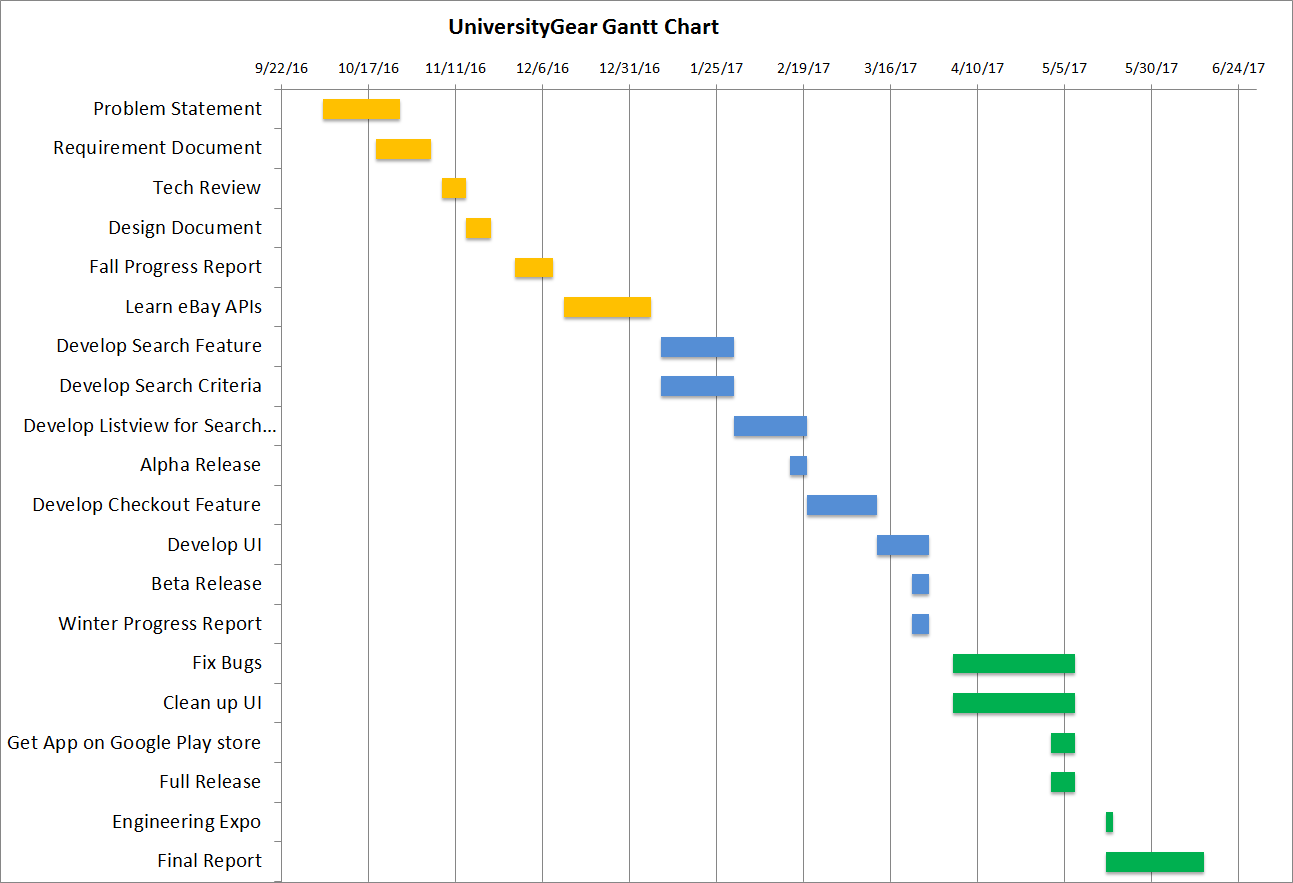
\includegraphics[angle=90,scale=.60]{ganttChart}
\end{figure}
\FloatBarrier

\subsection{Requirement Results}
Here are the requirements, as well as what happened to each one.
\begin{table}[!h]
\centering
\caption{The result of each requirement}
\label{Final requirements}
\begin{tabular}{l|l|l}
\hline
\textbf{Requirement} & \textbf{Completion} & \textbf{Comments} \\ \hline
Download application & Uncompleted & This went uncompleted because of time constraints.
\\ & & This requirement was also not important, especially when compared to the 
\\ & & others. \\ \hline
Update application & Uncompleted & This is due to the same reason above. \\ \hline
Determine search criteria & Completed & The search criteria was determined by  using common
\\ & & search filters, i.e. price range. \\ \hline
Guest checkout & Completed & The user can purchase items within the app. \\ \hline
Display search results & Completed & The user can browse search results within the app.
 \\ \hline
Display search results (no results found) & Completed & When no results are found, there will 
be an error message. \\ \hline
Item view for a selected item & Completed & When an item is selected, the user can view it 
in greater detail within app. \\ \hline
Save search criteria & Completed & When a user makes a search, it will save the schools they 
have search for. \\ \hline
Search feature performance & Completed & The search feature is the first thing the user 
is introduced to. \\ \hline
Usage of search feature & Completed & The feature offers many categories and filters, 
making for easy use. \\ \hline
Usage of search results in a ListView & Completed & Adequate information is provided to 
the user. Things like an image, price, 
\\ & & and title are given to them. \\ \hline
Usage of purchase feature & Completed & The user is notified that their purchase has 
been completed and they \\ & & received an order number. \\ \hline
Connectivity measurement & Completed & When they aren't connected to the internet, 
a message box tells them \\ & &  they need to be connected to use the app. \\ \hline
\end{tabular}
\end{table}

\subsection{Changes to the requirements}
There were no changes made to the initial requirements document. However, 
there are requirements that we did not meet. Unfortunately, the team had run 
out of time in order to complete these requirements. The two that will be 
uncompleted are getting the application to the Google Play Store, and Updating 
from the Google Play Store. These requirements were more of a ''soft'' 
requirement and were they did not take top priority. They didn't need to be 
explicitly completed throughout the course of the year, and could be completed 
after the school year. It should also be noted that our development times were 
completely changed, and that is reflected in the new Gantt chart below.

\begin{figure}[t]
This is what actually ended up happening during development.
\centering
\caption{Final Gantt Chart}
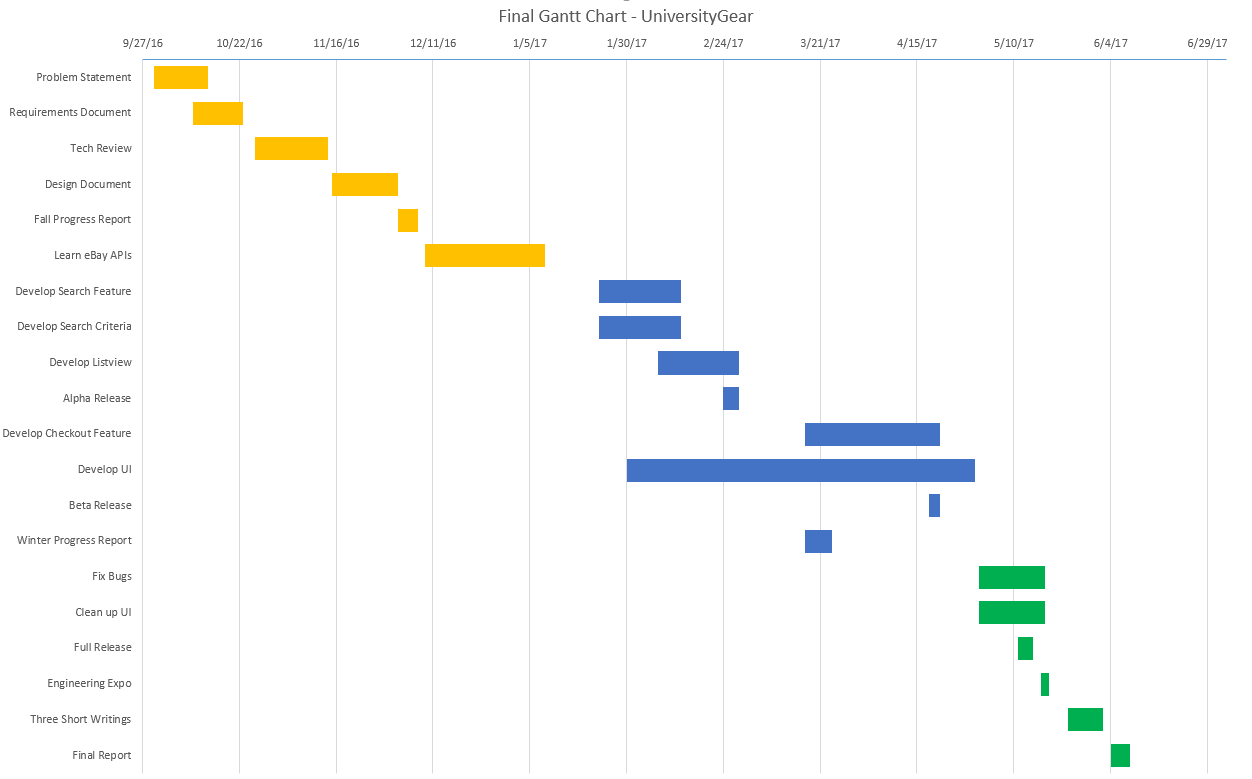
\includegraphics[angle=90,scale=.60]{finalGanttChart}
\end{figure}
\FloatBarrier

\section{Design}
\subsection{Introduction}
\subsubsection{Scope}
The application that is going to be developed will be for Android devices, 
specifically for N and M OS. It will allow users to purchase college merchandise
 via eBay's large collection of items. The user will be able to search for items
 from different colleges or by specific search criteria. The project will begin 
development in December, 2016 and end in May, 2017.

\subsubsection{Purpose}
The purpose of this design document is to outline how the application will be 
structured to satisfy the requirements we have set. It will go into depth about 
the design details of our software.

\subsubsection{Intended Audience}
The intended audience is for the team "4Credit" and their client. It is also for
 the professors of the senior capstone class at Oregon State University.

\subsection{Definitions}

\begin{table}[!ht]
\centering
\caption{Definitions}
\label{Definition Table Design Document}
\begin{tabularx}{\textwidth}{l|X}
\hline
\textbf{Term}               & \textbf{Definition}                              \\ \hline
API                    	      & Application Programming Interface, allows developers 
to develop applications that connect to eBay's large inventory of items. \\ \hline
Vendors               	      & Individuals or companies that sell or will sell items 
on eBay   \\ \hline
Filters                	      & Search criteria that will allow the user to more easily find 
the item that they are looking for.  \\ \hline
Third-Party Developers & Individuals outside of eBay that will be using eBay's public
 APIs to create their own applications.   \\ \hline
Application & An Android application that uses eBay's public APIs. \\ \hline
College Merchandise     & Items such as school supplies for Higher Ed, fan gear,
 etc...     \\ \hline
User                   	      & Any one who will be using the Android Application utilizing
 eBay's APIs.   \\ \hline
Client                 	      & eBay             \\ \hline
BIN                    	      & Buy It Now        \\ \hline
N                   	      & Android's new Nougat operating system 
\\ \hline
M                   	      & Android's Marshmallow operating system\\ \hline
MVC                   	      & A design pattern called Model View Controller
\\ \hline
\end{tabularx}
\end{table}
\FloatBarrier


\subsection{Conceptual model for software design descriptions}
The basic concepts and context of the design document will be explained in this 
section of the document.

\subsubsection{Software design in context}
An object oriented approach will be taken and we will be using a specific 
design pattern called MVC. This will allow us to maintain some form of a 
separation of concerns. In turn, it will make development much smoother. We will
 also have to keep track of an API layer, as we will be using eBay's new APIs. 
It is imperative that our application also works on the M and N Android 
operating systems.

\subsubsection{Software design descriptions within the life cycle}
\subsubsection*{Influences on design document preparation}
The software requirements specification (SRS) plays a large role in influencing 
the design document. This is because the SRS defines all of the functional and 
interface requirements for the successful completion of the project.

\subsubsection*{Design verification and design role in validation}
Test cases will be developed simultaneously to development phase. This will 
allow us to validate that our application is successfully working as expected. 
The last step of validation we will complete if our application successfully 
met the requirements defined in the SRS.


\subsection{Design description information content}
This section of the design document will identify how the application will be 
implemented and designed. 

\subsubsection{Design document identification}

\subsection{Design stakeholders and their concerns}
The stakeholders of the project our the developers and their clients. The 
biggest concern is that the product will meet all of the requirements specified 
in the SRS. The application must also contain design that is described in this 
document. 

\subsubsection{Design views}
We will be using different processes for representing diagrams. We will be using
 UML for describing our functions and classes.

\subsubsection{Design viewpoints}
The design viewpoints will be described with a combination of UML diagrams and 
short descriptions. The descriptions could include information regarding the 
context, composition, logical, or interactive viewpoints. Each viewpoint will 
also have a specific name.

\subsubsection{Design elements}
There are a lot of design attributes we will be discussing in our document. Our 
design entities will consist of the APIs and classes that we will be using to 
accomplish our goals. Each entity will have a name, a type, and a purpose. The 
name attribute is simply the name of the element or entity. The type attributes 
will consist of what kind of class or API we will be using. The purpose attribute 
is to give a description as to why an element might exist. Last, an author 
attribute will be used to identify which designer will be responsible for the 
element.

\subsubsection{Design rationale}
It is important that our application performs well on the N and M Android operating 
systems. We will make sure that the application is also easily maintainable 
for future developers. We will also provide documentation of the design process 
so that other developers will understand the structure of the application.


\subsection{Design viewpoints}
The main design viewpoints will be explained here. The exact viewpoints are the 
context, composition, logical, dependency, interfaction, and algorithm viewpoints.

\subsubsection{Context viewpoint}
The context viewpoint will document the functionality between the user and the 
application. There are two main functionalities the user should be using: 
searching and purchasing merchandise. This sections serves to define the user 
interaction with the app. It will also talk about the sub functions that will 
be used to facilitate the main functions. \newline

The user of the application will also have to perform other smaller actions in 
order to get the full use. For example, they will have to download the application 
from the Google Play store. From there, they would be required to search for 
something in order to purchase it. They will be searching for specific schools, 
prices, condition of item, and other search criteria. They will then be presented 
with a list of items in which they will be able to select and view that item in 
greater detail. They will also be able to purchase the item and then they will 
need to enter in their name and shipping information. \newline

When viewing an item in greater detail, the user will be given the opportunity 
to purchase the item. They will have to provide the application with some user 
information, such as a credit card number and shipping address. The user will 
also have to provide other information such as the school they are searching 
for, what item they are looking, the price of the item, condition of the item, 
and other filers of that sort.

\subsubsection{Composition viewpoint}
The application will be divided into three different parts. The first being the 
search feature, which will allow the user to find a specific item. The second 
will be the purchasing feature, which will allow the user to purchase any item 
they have found. Last, the user should be able to view in detail everything 
about the item they have searched for. All these pieces need to be connected 
together and coherently function as one piece. 

\begin{figure}[h]
\centering
\caption{UML Diagram for the for main classes}
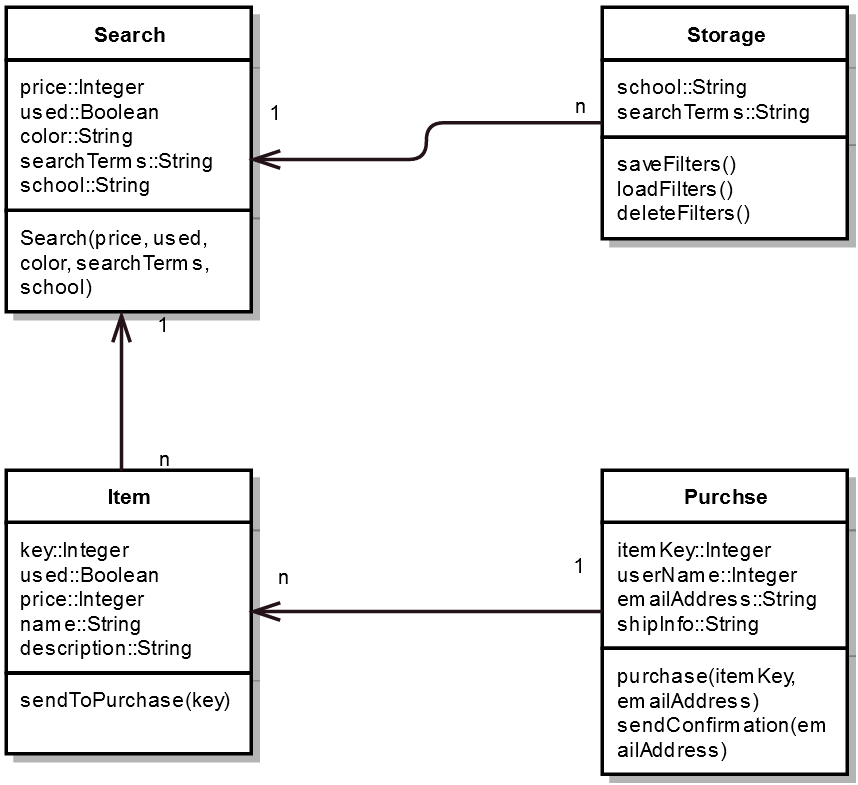
\includegraphics[scale=.65]{projectUML}
\end{figure}
\FloatBarrier

\subsubsection*{Function attribute}
The search class will allow users to search for their items. This class will need 
several variables, which will be passed into a function that calls an API. The 
output will be a list of items that are related to the search criteria provided 
by the user. The author of the search class will be Bryan Liauw. 
The storage class will allow the user to save their search filers 
for later use so they don't have to keep entering the same data each time. This 
requires the same information provided to the search. From there, the class will 
either save, load, or delete this data. Bryan will also be the author of the storage 
class. The item class will be used to hold and 
send the specific item data to the purchase class. Devin Foulger will be the 
author of the item class. The purchase class will allow 
the user to purchase the item that they have selected. It will also send a 
confirmation if the user's purchase has been completed. Devin will also be the 
author of the item class.

\subsubsection*{Subordinates}
The search class will be the default class that will control the application. 
This is because the storage and item classes will depend on the search class 
as you need to search for something in order to save the information and create 
items. The purchase class will depend upon the item class. This is because if 
are no items, then there will be nothing to purchase. In order to purchase 
something, an item must exist. 

\subsubsection{Logical viewpoint}
Our application will consist of many classes, but they will either be a model or 
a controller. These classes will be the Search class, Purchase class, Item class, 
and the Storage class.

\subsubsection*{The search class}
This class will allow users to search for items that they would like to view or 
purchase. It will share a relationship with the item and storage classes. It 
will have a method for searching that needs the search terms that have been 
provided by the user. The important thing to notice, is the variables provided 
by the user. These variables are the "price", which is a integer. The second is 
the condition of the item, which is called "used" and it is a boolean variable. 
The third variable is the color of the item and is named "color", which it is a 
string value. "searchTerms" is another variable of type string, and is used to 
hold the search values the user provides. The last variable is the "school" and 
is a string. The search method for this class also heavily relies on an API 
called "Browse" which is provided by eBay. \newline

The search class will now encompass the storage class. 

\begin{figure}[h]
\centering
\caption{UML for the search class}
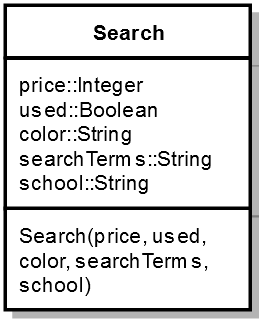
\includegraphics[scale=.9]{searchUML}
\end{figure}
\FloatBarrier

\subsubsection*{The storage class}
This class will be used to save the users search criteria. This is so the user 
will not have to enter in the same information again, considering that they 
will most likely search for the same schools over and over again. It will have 
the ability to save, load, and delete filters. It will also need the information 
provided by the user such as the school and searchTerms. Those variables will be 
provided by the search class. \newline

The storage class will no longer be used. This is because the methods involved are 
small enough that they can be condensed into the search class. The only place 
that these methods would be used is in the search class and because of this, we 
decided to condense the two. 

\begin{figure}[h]
\centering
\caption{UML for the storage class}
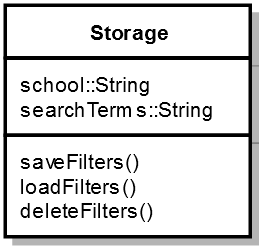
\includegraphics[scale=.9]{storageUML}
\end{figure}
\FloatBarrier

\subsubsection*{The item class}
The item class will hold all the information on a single item. The items will be 
displayed to the user in either a list view or a single item view. The information 
will also be sent to the purchase class so that the user may be able to purchase 
the item. This class heavily relies on what is returned by the search class and 
the Browse API. Every item will have a unique "key", that is an integer value. This 
variable exists so that every item that is in eBay's database has a unique 
identifier. The item will also contain a "used" variable that will be a boolean 
to determine if the item is used. The "price" will be an integer variable that 
determines how expensive the item is. It will also have a "name" and a 
"description" variables,  both will be strings. The "sendToPurchase" method will 
allow users to purchase the item that they have chosen. This means that the key 
will be needed for this transaction to take place. The key will identify which 
item is being purchased. The item class will also need to use the Android JSON 
parser. This is because the returned value from the search from eBay's Order 
API is a JSON file. The JSON parser will need to be able to parse the file for the
correct information.

\begin{figure}[h]
\centering
\caption{UML for the item class}
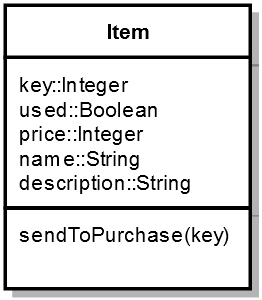
\includegraphics[scale=.9]{itemUML}
\end{figure}
\FloatBarrier

\subsubsection*{The purchase class}
The purchase class will allow the user to purchase the item that they have 
selected. It will need the item key when purchasing an item. It will also notify
the user in some way that they know the purchase has been completed. The first 
variable that is needed is the "itemKey", which is a unique key that identifies 
which item is being purchased. The next variable, is the "userName", which will 
hold the users first and last name. The third variable is a string called 
"emailAddress" that will hold the user provided email address. The last variable, 
"shipInfo" will hold the users shipping address. The "purchase" method will 
require the use of eBay's "Order" API. The purchase method will also need the 
email address. 

\begin{figure}[h]
\centering
\caption{UML for the purchase class}
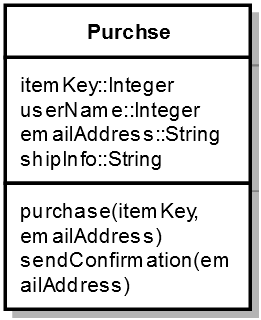
\includegraphics[scale=.9]{purchaseUML}
\end{figure}
\FloatBarrier

\subsubsection{Dependency viewpoint}
Each class is somewhat dependent on the search class, as it is the basis of 
where everything starts. Item and storage can only exist after something has 
been searched for. The purchase class can only exist if an item exists.

\subsubsection*{Search class dependencies}
The search class does not depend on any other classes in order to function. 
However, it does depend on eBay's Browse API. This API is what will give us the 
ability to search for items.

\subsubsection*{Storage class dependencies}
The storage class depends on the search class. It also depends on what 
information has been provided by the user. The purpose that the storage class 
depends on the search class, is because it needs to save specific information 
such as the school and search terms. The search class also contains the information 
that has been provided by the user, which the storage class will need. 

\subsubsection*{Item class dependencies}
The item class depends on the storage class. This is because it will need 
the information that is returned from the item search. The purpose that this 
class depends on search is because the item will need the information that is 
returned from the search method in the search class. It also depends on the 
Android JSON parser. This is because the returned value from the search method 
will be in a JSON format. The JSON parser API will need to correctly return the 
required information for the item class.

\subsubsection*{Purchase class dependencies}
The purchase class depends on the item class. The class will need the 
information that is in the item class, like the item key. The purpose that this 
class depends on the item class is because purchasing needs the item key. The 
purchase class will also depend on eBay's Oder API. EBay's API will allow the 
class to make its purchase. The API will also need the item key. 

\subsection{Interaction viewpoint}

\subsubsection*{Home Page}
The home page will be a simple design that will include a search bar labeled 
'searchText' and a button 'searchButton' for the user to enter text and 
submit their search. When the user presses the search button, the text within 
the search text field will be passed as a string parameter to the search method.
The user will not be allowed to press the search button without first inputting 
text into the search field. To submit a search from the home page, the user will 
also be allowed to use the search button on the on-screen keyboard. 

\subsubsection*{Multi List View}
This module will proceed the home page, after the user searches for an item. 
After the search module completes its search, it will return a list of data 
structure that contains the search results. The pertinent information in the 
search results will consist of an image of the item for sale, the item name or 
title, and the item price. The DisplayResults module will then take these 
results and present them to the user in a list view. \newline

The image that will be displayed in the list view will be a smaller version of 
the main image. This will be done by the service that will be used by the 
search module. The image size reduction will be necessary to reduce loading 
times and thus performance impacts. \newline

In this same multi list view module, there will be a filter component that will
 allow the users to filter the search results. The users will be able to filter 
the results based on predefined criteria. The currently defined search filters 
include price (Integer), item category (String), or item condition (new or used) 
(Boolean). These details regarding an item will be part of the data that is 
returned by the search module but not displayed to the user until they enter 
the single item view.

\subsubsection*{No Search Results}
If after the user submits their search, or modifies their search criteria to the
 point that there are no search results to display, this module will present a 
message stating that there are no search results and to try a different search, 
or to modify their search criteria. This module will be based off the size of 
the list returned by search.

\subsubsection{Algorithm viewpoint}
The algorithms viewpoints will describe the different algorithms that we will be
 using to correct users search mistakes. The Levenshtein Distance algorithm that 
we are going to use is going to be attached to the search bar that is in most 
pages of the UI. The algorithm will run every time the users finish typing and 
submitting their search. The algorithm will run regardless whether the keyword 
needs to be corrected or not. The fix will happen if the user has written 
something that is not quite correct; that is, the distance between the intended 
string and the string that user has written does not have a 0 value. Once this 
case happens, we will find the keyword with the minimum distance from the string 
user has written and replace user's keyword with that.

\subsubsection*{Design concerns}
There is a huge concern in terms of resources needed. Since the algorithm is 
going to compare keywords from the user to keywords in the database, this 
means that the algorithm will run once for every words in the database. 
Furthermore, the algorithm itself has a complexity of O n-squared, since the 
number of loops is the string size of one string times the string size of the 
other. This means that the total complexity would be O n-cubed. One way to get 
around this is to find a threshold. Once this threshold is reached, the word 
is considered similar enough. This can reduce a lot of processing time.

\subsubsection*{Processing attribute}
This algorithm will be part of the search method inside the search class. 
Because of this, it will affect only the variables within the class. 
Since we are correcting the users input string, we will use the algorithm to 
manipulate the variable color, school and searchTerms. The fixing price and used 
variable is unnecessary, because it does not need to be fixed. The only thing 
we could do to price is find the approximate integer to the user's input, while 
the used variable should not be modified. The algorithm will find the most 
similar string based on the differences in the character in each position. 
This is done by constructing a two-by-two matrix and then filling it with an 
integer based on a certain rule. This rule will measure the differences 
between the characters in each string and assign an integer to determine how 
different it is. As previously mentioned, the loop happens every time user 
enters a keyword. Once the keyword is entered, the algorithm will run until 
it reaches a string distance that is below or equal to the threshold.

\subsubsection*{Examples}
\begin{lstlisting}
LevenshteinDis(string1, string2){
	Matrix[string1.length][string2.length]
	for(a = 0 to string1.length){
		for(b = 0 to string2.length){
			if a==b{
				if string1 at a = string2 at b
				   Matrix[a][b] = 1
				else 
				   Matrix [a][b] = 0
			}
			else 
			   min(Matrix[a-1][b]+1, Matrix[a][b-1]+1, Matrix[a-1][b-1]+1)
		}
	}
}
\end{lstlisting}

\subsection{Changes to the design document}
The design document went through very little in change. There was only one small modification
that was made to the system that we had come up with. We discovered that saving the specific
colleges that users have searched for didn't need its own class. The method was small enough
that it could be stored in the class that was calling it. In the design document, we explain
why we made this change in greater detail.

\section{Technologies}
\subsection{Introduction}
Our team, 4Credit (team number 6), will be developing the application UniversityGear. 
This application will allow users to browse eBay's catalog and purchase items 
related to college merchandise. Devin will be in charge of creating a way for 
users to checkout, developing the UI for it, and getting the data for items to
be displayed in a single item view. Bryan is in charge of correcting the user's 
search keywords, searching for items in eBay's database, and saving search 
filters for later use by the user. Hector will be in charge of creating a list to 
view items in a list, handling when no search results are found, and creating
a home page. Devin and Hector will have the same role of client interaction and
development. Bryan will be the back-end developer.

\subsection{Technologies}
\subsubsection{Technology: Checkout}
Checking out is a feature that is essential to any application or website where
you purchase some item. This means that our application will need to allow the
user to check out the items in some fashion.

\subsubsection*{Options}
\subsubsection*{Option 1: Checkout with sign-in}
Allowing the user to sign in to checkout items gives us the benefit of allowing
members to purchase from our application. In order to implement this feature, we 
would have to use eBay's Order API. This API would allow for the user to
purchase items using their existing eBay and PayPal accounts. This also allows
the user to view the shipping address provided and any fulfillment information.

\subsubsection*{Option 2: Checkout as guest user}
Allowing the user to checkout items through a guest check out would allow any
user to purchase from our application. In order to implement guest checkout, we
would need to use eBay's Order API with GUEST CHECKOUT SESSION. This is
different than using the Order API normally. With guest checkout, the user is
able to see that item that they have purchased and the status of the payment and
 order.

\subsubsection*{Option 3: Checkout as either guest user or with sign-in}
Allowing the user with the option to either sign-in or use guest checkout gives
us the option to offer which ever method makes the user most comfortable when
checking out. This would be that we would have to use eBay's Order API to the
fullest by implementing both sign-in and guest checkout. This means that the
user would be able to use PayPal, if they have an account, or checkout via
credit card.

\subsubsection*{Use in design}
This is a fundamental use in our design. Without this feature, or application
would simply be a searching application. The user would only be able to search
for specific items that exist within eBay's stores, but not actually purchase
them.

\subsubsection*{Cost, availability, speed, security}
\subsubsection*{Option 1: Checkout with sign-in}
The cost of checkout with sign-in is the development time it would take to
implement. This feature is tricky and would complicates the use of eBay's APIs.
However, the availability is limited to those that have an eBay account. The
speed is also largely dependent on internet connectivity and the status of
eBay's servers. Finally, the security is very tight. This is because the user
must authenticate before making a purchase. On top of that, all information that 
is used is sent via HTTPS.

\subsubsection*{Option 2: Checkout as guest user}
The cost of guest checkout is relatively low. It would take the least amount of
development time and resources. The availability is also very high allowing us
to reach anyone who would like to use our app. Again, the speed is dependent on
internet connectivity and the status of eBay's servers. However, the security
would be great. None of the user's information should be saved to the device.
That includes things like credit card information and shipping address. Also,
any information that is used is sent via HTTPS requests.

\subsubsection*{Option 3: Checkout is either guest user or with sign-in}
The cost of the guest checkout coupled with sign-in is very high. It would
require a significant amount of development time to complete. However, the
availability would be at its greatest because it would allow for any and all
users to purchase items. The speed of the checkout would, again, depend on the
status of eBay's servers and internet connectivity. The security is the same as
the above options.

\begin{table}[!h]
\centering
\caption{Comparison Table of Options for Checkout}
\label{Comparison Table of Options for Checkout}
\begin{tabularx}{\textwidth}{|l|l|l|l|X|}
\hline
\textbf{} & \textbf{Time Cost} & \textbf{Availability} & \textbf{Speed} &
\textbf{Security} \\ \hline
\textbf{Option 1} & High & To only members of eBay & Fast & Best, because it
offers an extra layer of authentication \\ \hline
\textbf{Option 2} & Low & To everyone as a guest & Best & Great \\ \hline
\textbf{Option 3} & Very high & To members of eBay and guests & This could
either be best or fast & This could be best or great \\ \hline
\end{tabularx}
\end{table}

\subsubsection*{Evaluation}
Each option has their advantages and disadvantages. If we were to allow users to
 checkout only using sign-in, then we might only be targeting a smaller audience.
 The complexity for implementing such a feature is much harder than that of 
guest checkout as well. Using guest checkout would allow for all users to use our
application with no complicated sign in. It would also mean that users would not 
have to create an account to user our application. If we were to implement both
sign-in and guest checkout, the complexity would be too great. Given the small
amount of development time it might be hard to implement both features. 
However,this option would give us the ability to reach every user possible.

\subsubsection*{Best Choice}
The best choice for our application is implementing a guest checkout. This is
because with a short development time, guest checkout would be the fastest to
implement. This would also allow any user to purchase from our application,
which means we would not be alienating someone who does not have an eBay
account.

\subsubsection{Technology: Checkout UI}
Checking out needs to have a UI that is easy to use. If we only stub out a UI,
it might be complicated, or worse, ugly. The UI needs to be attractive and
functional.

\subsubsection*{Options}
\subsubsection*{Option 1: Layout Editor (Native Android Studio)}
The native android layout editor doesn't work very well for prototyping.
However, it allows for easy UI creation while being able to map the buttons to
correct functions. This tool doesn't offer much in terms of quick design, but it
offers a lot of functionality. It uses XML files to create the UI. It does allow
you to alter any aspect of your UI, which is very good as well. It also allows
you to create your own UI objects very easily.

\subsubsection*{Option 2: Indigo Studio}
Indigo Studio is a wire framing tool. With this tool I would be able to create
great looking wireframes. This doesn't allow for much in terms of actual
development though. It is just a tool for quick prototyping and design. However, 
it does offer a lot in terms of customization and they also offer a lot of
images for buttons, list views, and things of that sort.

\subsubsection*{Option 3: Just In Mind}
Just In Mind is a comprehensive prototyping tool for many types of development,
including Android development. This tool offers a lot in terms of development.
There are many UI libraries for Android. This tool would also allow me to use
templates that they have already built. On top of that, any of the designs or
UIs I make can be transferred into already existing projects. This tool also
offers integration with other tools as well, like Photoshop. It also features
interactive images and animations for use in your projects.

\subsubsection*{Use in design}
Having a functional and beautiful looking UI keeps users attracted to your app.
So, having a nice UI is a must in this project. The user will also constantly be
interacting with the application.

\subsubsection*{Cost}
These tools are simply for creating clean and responsive UIs. That being said,
the native Android Studio Layout Editor is free. Indigo Studio costs 25 dollars
a month and Just In Mind costs 19 dollars a month.

\begin{table}[h]
\centering
\caption{Comparison Table of Options for Checkout UI}
\label{Comparison table for checkout}
\begin{tabularx}{\textwidth}{|l|l|X|}
\hline
\textbf{}         & \textbf{Cost}                & \textbf{Learning Curve} \\ \hline
\textbf{Option 1} & Free                                                & There
is somewhat of a learning curve as it requires you to also develop at the same time \\ \hline
\textbf{Option 2} & Free with limited features, then 25 dollars a month & Low \\ \hline
\textbf{Option 3} & Free with limited features, then 19 dollars a month & Low \\ \hline
\end{tabularx}
\end{table}

\subsubsection*{Evaluation}
Each tool has clear disadvantages and advantages when compared to each other.
Just In Mind and Indigo Studio have relatively similar functions. However, Just
In Mind offers a bit more such as UI libraries that are compatible with Android
Studio. Indigo Studio does allow for faster creation of wireframes when compared
to Just In Mind. These two tools can be much better than the native layout
editor in Android Studio. The editor layout also offers its own features as
well. It gives developers the ability to customizing anything they like about
their UI.

\subsubsection*{Best Choice}
The best choice for this project would be to use the native Android Studio
Layout Editor. Although the other tools offer a lot more in terms of
prototyping, they have a cost. If you don't pay for the tools, you don't get
everything that is included. However, Android Studio does offer the ultimate
tool for any type of customization you would like to make. You have full control
over what you are trying to do. You also don't have to worry about integration
with other tools, because it is built in.

\subsubsection{Technology: Getting data for Single Item View}
The data that is received from eBay's APIs comes in the form of an JSON file.
This JSON data needs to be parsed correctly so that the information is portrayed
to the user in a meaningful manner. Each item needs to correctly be displayed to
the user so that they can view the description or images of a particular item.

\subsubsection*{Options}
\subsubsection*{Option 1: }
GSON allows for Java objects to be converted into JSON objects, and vice versa.
This is a tool that is not native to Android Studio, but offers a lot in terms
of use. It has many methods that allow for array creation which holds JSON
information. These arrays can then be used to fill the UI with relevant
information for the user to view.

\subsubsection*{Option 2: }
JsonReader is a light weight API that would allow me to easily read JSON files.
It allows me to create JSON objects and arrays. The arrays would hold
information that could easily be presented to the user.

\subsubsection*{Option 3: }
JSON Parser is native to Android Studio and is very comprehensive. It would
allow me to create objects using JSON files. I would have the ability to create
JSON arrays, object, and key-value pairs using JSON Parser. It includes many
methods for easy creation of JSON objects and parsing.

\subsubsection*{Use in design}
A JSON parser is absolutely a must if we want to make sense of our data. This is
because eBay's APIs return the data in JSON format. In order to display the
information correctly to a user, we have to use a JSON parser.

\subsubsection*{Cost and speed}
All three APIs do the same thing in the same fashion. They all create readable
JSON arrays that hold information to be used by the developer.

\subsubsection*{Comparisons}
All three APIs do the same thing in the same fashion. They all create readable
JSON arrays that hold information to be used by the developer.

\subsubsection*{Evaluation}
It is important to note that theses APIs perform almost identically. On top of
that, they all produce the same output. There is no clear advantage or
disadvantages over the others. The only disadvantage to the JsonReader, is that
you don't have the ability to create new JSON objects.

\subsubsection*{Best Choice}
The best choice to use for our application would be the built in Android parser,
JSON Parser. This is because all the parsers perform similarly, but with the
built in parser, I get to avoid the headache of importing a new one. It also has
the ability to create new JSON objects if that is needed.

\subsubsection{Technology: Correcting User's Search Keyword}
Sometimes, when a user wants to find an item, he/she will mistype what they want to
search. This is a more prevalent issue in mobile apps since the keyboard input is
much smaller in smart phones. If we do not address this issue, the return value from
the search will not be optimal. In order for our app to understand what the user
wants to find despite the misspelled keyword, we need a fuzzy search algorithm.
There is 3 fuzzy search algorithms that comes into consideration: Levenshtein
Distance, Hamming Distance and Metaphone.

\subsubsection*{Options}
\subsubsection*{Option 1: Levenshtein Distance}
Levenshtein Distance calculates the similarity of two strings and assign a numerical
value that determine how different the two strings are. This algorithm, given a
string s and a target string t, will return the number of alterations to s so that it
will be the same as t. The algorithm will construct a matrix m which has the size
m[s.stringlength][t.stringlength]. The matrix will be built on the minimum from this
rule:

\begin{lstlisting}
	1. If s[n] == t[n] where n is != t.stringlength 
		m[n][n] = 0 
		else if s[n] != t[n] 
			m[n][n] = 1
	
	2. m[a][b] where a < s.stringlength and b < t.stringlength 
		=  m[a-1][b]+1 or m[a][b-1]+1 
	whichever is smaller
	
	3. m[a][b] where a < s.stringlength and b < t.stringlength 
		=  m[a-1][b-1]+1
\end{lstlisting}

\subsubsection*{Option 2: Hamming Distance}
Hamming Distance is another algorithm that compares the difference between two
strings and assign a numerical value on how close one string is from another.
However, unlike Levenshtein Distance, the Hamming assigns value similar to a binary.
This algorithm will create an array of integer with the size of the length of the
string. This array's value at a given position n is 1, if the character of the first
string and the second string at n is the same, or 0 otherwise. The array's value is
totaled up and it will give a value on how different one string is from another.

\subsubsection*{Option 3: Metaphone}
Metaphone, on the other hand, does not assign a numerical value to check the
difference. It mainly checks if some character is substituted with its homophone. For
example, the algorithm will consider K and C similar and so is "kall" and "call".

\subsubsection*{Comparison}
The main criteria that we evaluate is the reliability of the algorithm to find what
the user might mean when they accidentally mistyped a word. Secondary criteria
include maintainability and speed.

\begin{table}[h]
	\centering
	\caption{Comparison Table for the Fuzzy Search Algorithms}
	\label{Comparison Table for the Fuzzy Search Algorithms}
	\begin{tabularx}{\textwidth}{|l|l|l|X|}
		\hline
\textbf{} & \textbf{Reliability} & \textbf{Maintainability} & \textbf{Speed}
		\\ \hline
		\textbf{Option 1} & Applicable to most cases & Easy to maintain & Slower
		\\ \hline
\textbf{Option 2} & Applicable to most cases except non-equal string & Easy to
maintain & Fast
		\\ \hline
\textbf{Option 3} & Not applicable in most cases & Harder to maintain & Fast		\\ \hline
	\end{tabularx}
\end{table}

\subsubsection*{Best choice}
For our application, Levenshtein Distance is the best option. Metaphone does not take
into account if user's input is not homophone to what the user wants to find. This
might be a problem if user is searching for certain types of brand. Also, adding
language support in the future means that we need to change some parts of the code to
cater to the new language since there will be different pronunciation. We will need
to change how our algorithm detect homophone if it happens and it will take
unnecessary time. On the other hand, the Hamming Distance is a faster algorithm than
Levenshtein since we only need to construct one-dimensional array as compared to
Levenshtein's two. But, Hamming Distance cannot give an accurate number if the length
of string is not equal. This can happen in the application if the user accidentally
sends in an incomplete keyword or simply do not know the exact keyword he/she is
looking for. Despite the trade-off in speed, we believe that Levenshtein's
reliability is more suitable for our application in order for user to have an optimal
session.

\subsubsection{Technology: Search Item in eBay's Database}
User will be able to find certain items in the application. The user will be able to
enter keyword and the app will return items that matches, or approximately matches,
user's query. This search result will be used alongside filters in order to get the
exact item that user wants.
The 3 ways we can go around this search is: Binary Search, Linear Search, eBay's
Finding API

\subsubsection*{Options}
\subsubsection*{Option 1: Binary Search}
Binary search involves dividing the array into multiple halves until a match is
found. If the item to be searched is larger than the middle value, then the top half
will be the half to be searched. Else, the lower half will be searched. This search
algorithm's complexity is log n since the array size is halved every iteration. It is
considerably fast, especially when used in a larger database. However, the main
drawback is that the list must be sorted for this to work. Without a sorted list,
dividing the halves would not help finding the item since the top half and lower half
might not be larger or smaller respectively.

\subsubsection*{Option 2: Linear Search}
Linear Search is one of the most basic search. This involves checking every item in
the list and find if it matches the item. This algorithm's complexity is n since it
will look for every item. Considering the complexity, the speed of the algorithm is
slow especially in larger files. While smaller database would mean unnoticeable
difference in speed, it is very unlikely that our application will utilize small
database. The advantage of linear search is that there is no need to manipulate the
list of data we are looking in. Since the search will iterate over every single item
and match it with the keyword, there is no need to sort like binary search.
Therefore, despite the trade-off in speed, linear search makes it up with
reliability.

\subsubsection*{Option 3: Ebay Finding API}
eBay has a released API that search their database. It has a lot of function that
helps finding based on the query. Furthermore, it has several functions that helps
narrow down user's selection through filters. Despite not being transparent in how
their search works, eBay does widen the way a query can be searched, such as by
product or by keywords. As a bonus. the eBay API helps in manipulating the way search
results are returned. Since we are going to use eBay's sell and buy API, this API
will integrate well with other APIs.

\subsubsection*{Comparison}
The main criteria are speed and reliability. Some other consideration would be
integrating the result with other functions later.

\begin{table}[h]
	\centering
	\caption{Comparison Table for the Search Algorithms}
	\label{Comparison Table for the Search Algorithm}
	\begin{tabularx}{\textwidth}{|X|X|X|}
		\hline
		\textbf{}         & \textbf{Reliability}                & \textbf{Speed} 
		\\ \hline
		\textbf{Option 1} & Low & Fast
		\\ \hline
\textbf{Option 2} & High & Slow		\\ \hline
\textbf{Option 3} & High &Fast(?)		\\ \hline
	\end{tabularx}
\end{table}

\subsubsection*{Best choice}
We believe that the best approach would be using the Finding API. Since we are using
eBay's database, we have no guarantee that it would be sorted, therefore making
binary search a risk. On the other hand, if it is sorted, using a linear search would
make it run slower. We believe that the Finding API would be optimized by eBay and
will find the item fast and accurately. Furthermore, giving a lot of options such as
filtering will help us in the future. The integration with other API that we will use
is also a convenience that we should take advantage of.
  
\subsubsection{Technology: Saving Search for Future Purposes}
Our application will store user's search history internally in their phone. This is
so that we can give an accurate recommendation of items based on user's past search
history. The search history would be saved in a .txt format in the application
folder. There is two ways we can go around this: we can save the item id and search
it in the database in order to understand what the user's preferred item is or we can
save the keywords and determine user's preference through those keywords.
There is 3 ways we can save this txt file: Internal storage, External Storage, or
Server

\subsubsection*{Options}
\subsubsection*{Option 1: Internal}
Internal storage means that the application would save user's preference inside their
mobile phone. This means that the user has total security from other source. Android
makes sure that the file saved internally is, under normal circumstances, only
accessible by the application itself. Furthermore, since the files are saved
internally, the application's read and write speed is faster by a certain margin;
most likely to be noticeable in lower-end hardware. However, the internal storage of
most Android smart phone is rather limited compared to external ones, therefore,
saving a huge file might frustrate the user.

\subsubsection*{Option 2: External}
Relying on external Storage using SD card or other similar hardware means we are
going to operate under the assumption that the user has such external storage. While
it is not an uncommon situation, some user might neglect having an external storage,
so it is not quite ideal. However, using external storage means high load of data is
possible. We would not worry about utilizing too much user's data. Although its read
and write speed will be slower, but having an external storage means that it is
possible to offload some processes to the memory card instead. However, security can
be easily compromised if the external storage is detached and lost. The data can
easily be retrieved once someone manage to get into the external storage.

\subsubsection*{Option 3: Server}
Using server will require internet connection. Given our application rely heavily on
internet, we can safely assume that user will have some kind of connection that
allows us to utilize an online database. By saving it into the server we do not need
to worry about the data load, since it is going to be handled elsewhere. The
trade-off would be the speed to process things, which is highly dependent on the
internet connection the user has. This can range from being very fast to very slow
depending on where the user is geographically.

\subsubsection*{Comparison}
The speed on which the file can be taken would be very important, because we might
need it for different purposes. If the speed is too slow, user might get the feeling
that the application is not responding fast enough, which is something we must avoid.
Secondary criteria would be security and storage space.

\begin{table}[h]
	\centering
	\caption{Comparison Table for the Storage Medium}
	\label{Comparison Table for the Storage Medium}
	\begin{tabularx}{\textwidth}{|X|X|X|X|}
		\hline
\textbf{} & \textbf{Security} & \textbf{Speed} &\textbf{Space} \\ \hline
		\textbf{Option 1} & Very Secure & Depends on the phone & Limited
		\\ \hline
\textbf{Option 2} & Not secure & Depends on the phone but slower than internal
Storage & Depends on the hardware but generally larger than internal storage
		\\ \hline
\textbf{Option 3} & Mostly very secure &Depends on the phone and internet connection
& Very huge but comes with a cost.
		\\ \hline
	\end{tabularx}
\end{table}

\subsubsection*{Best choice}
Our application will use the internal storage with the option to allow user to use
external storage. We believe that the speed on which the information is retrieved is
very important. The data we are going to put in is not going to be very large; if the
data gets too large, we will have to narrow it down by removing past searches to
indicate the user's changed preferences. Using a server database online would add a
different layer of complication and unnecessary because the data would be small in
size. Furthermore, we won't have any other operation on the data which makes it
unnecessary for it to be saved on a server. We respect the users and their security,
which is why we would try to use the most secure method possible. However, if the
user does not have enough space internally, we would give an option to trade that
security and speed for more space.

\subsubsection*{Optional Task: Machine Learning to Study User's Preference}
Once we have user's history of searches, our application should make use of that by
constructing user's preferences based on the information it stores. Additionally, we
can also use data that might be provided from the Ebay server to add more data in
order to get higher accuracy. This preference will be used for multiple purposes,
which can range from showing items on the home screen of the application, to
suggesting the user what to buy at the buying page. We construct this preference
using machine learning.
The 3 approach we can use to determine user's preference is Bayesian Estimate,
Apriori Algorithm, FP-Growth

\subsubsection*{Options}
\subsubsection*{Option 1: Bayesian}
Bayesian algorithm involves comparing whether one thing is going to happen following
a certain event or if another event is likelier. This is calculated by learning the
pattern to what is considered as true or false. In terms of this application, true
would be user''s preference. The algorithm counts the combination of prior events and
its results and construct a possibility based on a given event. Given high
possibility, we can assume that the user will want that item. This operation,
however, might be time-consuming because there is a lot of mathematical calculations
as well as receiving data.

\subsubsection*{Option 2: Apriori}
The Apriori algorithm calculates the most probable item or combination of items. The
algorithm involves counting the number of occurrences where each item is selected in
the data. Then, the number below a given threshold, which is usually half of the
number of data, is removed. Then each item is then paired together and we count the
number of occurrence where the pair is selected. Again, the number below the
threshold is removed. This keeps repeating until we decide to stop and we will get
the most probable item that user might want. Considering this, the running time might
be long because we need to iterate through the data every time we want a larger size.
Since we might also need a temporary storage for the lists, memory consumption might
cause lower-end smartphones to lag, something we want to avoid the user from
experiencing.

\subsubsection*{Option 3: FP-Growth}
Similar to Apriori algorithm, the algorithm will count the number of occurrences for
each item. However, instead of iterating and growing the items, FP-Growth will create
a tree based on the data given. Each item will be represented by a node. The node
will have a value on it which depends on how many occurrences. The node is going to
be connected based on the data; so given data set {1,2,3} and {1,5,6}, the tree will
branch out at item 1 and the value of the node at item 1 will be 2. The route with
the highest value will be the most probable outcome. This algorithm is significantly
faster than Apriori although it will not create as much possibilities.

\subsubsection*{Comparison}
The speed and the accuracy of the algorithm. Since slow algorithm will look
unresponsive, we would very much like to avoid that situation.

\begin{table}[h]
	\centering
	\caption{Comparison Table for the Machine Learning Algorithms}
	\label{Comparison Table for the Machine Learning Algorithms}
	\begin{tabularx}{\textwidth}{|X|X|X|}
		\hline
		\textbf{}         & \textbf{Accuracy}                & \textbf{Speed} 
		\\ \hline
\textbf{Option 1} & Accurate and can give lots of probable items & Slow, since it
might need to run through prior data several times
		\\ \hline
\textbf{Option 2} & Accurate and can give a lot of probable items & Slow, exponential
depending on how many iteration is needed
		\\ \hline
\textbf{Option 3} & Accurate but limited items & Fast, only requires at most 2 passes\\ \hline
	\end{tabularx}
\end{table}

\subsubsection*{Best choice}
We believe that FP-Growth might be the best choice. We value speed in our
application. User will feel that the app has too many loading times or unresponsive
if the algorithm takes much time. Considering the file might be larger as user uses
more of it, it is not recommended to use exponentially long algorithm.

\subsubsection{Technology: Viewing Multiple Search Results}
After a user submits a search, the API could potentially return hundreds of results
that will need to be presented to the user in an organized manner.

\subsubsection*{Options}
\subsubsection*{Option 1: Single item view with swiping}
We could present one item at a time which would allow us to present more details of
the item. To view more items, the user would swipe left or right to go through the 
rest of the items in the search results. This would also eliminate the need for the 
user to click on the item to view more details as the relevant details would already 
be presented. The user would have enough information to know if they want to 
purchase the item. The ``Buy'' button would be on this view to allow quick purchases. 
\subsubsection*{Option 2: Item list view with pages}

We could also present the items in a list view, that would display X number of 
results per page. The users would swipe up or down to browse through the different 
items presented. This view would provide minimal details such as a short item 
description, and a thumbnail image. There would be a ``Next'' and ``Prev'' buttons 
that would allow the user to browse through the rest of the results that are not 
already presented.

\subsubsection*{Option 3: Item list view without pages}
This would be like the previous, present the items in a list view. The difference 
would be that instead of browsing through several pages, once the user reaches the 
end of the search results that are present more results would load, if they're 
available. Otherwise a message would be displayed at the bottom of the page saying 
``There are no more search results''.

\subsubsection*{Use in design}
This is an important use as without a proper presentation of the search results, 
the users could get confused and frustrated to the point that they won't use the 
application.
\subsubsection*{Cost}
\subsubsection*{Option 1: Single item view with swiping}
This option would be implemented using Android Swipe Views that allow the users 
to motion left and right to browse through the search results. The speed impact 
using this implementation would be the cost of rendering all the details for each 
item. 
\subsubsection*{Option 2: Item list view with pages}
Implementing this option would be done using the built-in Android ListView 
activity. Speed would be reliant on the android device and internet connectivity 
to render the list of items to be displayed. The speed impact would not be as 
significant as option 1 as only the basic details re rendered for each item.
\subsubsection*{Option 3: Item list view without pages}
The cost of implementation for this option would be similar to that of option 2. 
The only difference is that more search results would render automatically when 
users scroll down to the end of the already displayed results. 

\subsubsection*{Evaluation}
All three options bring their own advantages to the table. The first option, will 
provide much more details regarding the items which is great. The drawback to 
option 1 is that it could potentially take much longer for the user to browse the 
hundreds of search results that are returned. Option 2 allows the user to set the 
number of results displayed per page. This allows the user to quickly browse through 
hundreds of items. Option 3 has some of the advantages of option 2, however users 
could get confused when they reach the end of the search results. The users would 
have to swipe down far enough for more options to be presented. If they don't, this 
could lead them to think that there are no more search results and think that the 
specific item that they are searching for is not available. 

After working on the project we have decided to use Option 3 and display all 
search results without requiring users to scroll through different pages. 
Since performance is not an issue, we will be loading all search results at 
once. Using option 3 eliminates the need for users to click on 
"Next" or "Prev" to go through the different pages of search results. Also, 
there will be no need for the user to scroll to a certain point for more 
results to load. 

\subsubsection*{Best Choice}
The best choice for the app is to use Option 2 where the results are presented in 
a list view with X number of results presented per page. This result is very 
similar to other apps that the user would likely have used. It's such a 
straightforward approach, that even if the user hasn't used a similar 
application, there should not be any confusing when browsing the results. 

\subsubsection{Technology: Handling No Search Results}
\subsubsection*{Options}

\subsubsection*{Option 1: Display message}
When there are no search results available, we could simply display a message 
that states ``There were no results found based off your search criteria. Try 
modifying your search criteria and try again.''
\subsubsection*{Option 2: Display alternate search results}
When there are no search results based on the provided criteria, we could 
modify the criteria and present search results for the modified search. When 
presenting these alternate search results, we would display a message that 
states what the search criteria is.
\subsubsection*{Option 3: Display alternate results based off search history}
If no items are returned for a specific search, the users could be presented 
with a history of their past searches. This could allow the users to revisit 
past searches that they may want to possibly continue.
\subsubsection*{Use in design}
While not the most critical piece of the system, the functionality will be part 
of the ``ease to use'' aspect of the app. Letting the user know that their 
search returned no results would be helpful in that the user would not have to 
guess why there is nothing displayed on the screen. They could wrongfully 
assume things such as the app has crashed or internet connection is not 
letting items load correctly.
\subsubsection*{Cost}
\subsubsection*{Option 1: Display message}
Cost of implementation would be minimal. A simple message notifying them of no 
search results would also be very Fast as it would not take much to render the 
message. 
\subsubsection*{Option 2: Display alternate search results}
This option would have a high implementation cost. We would need to determine 
the best method in which to modify the search criteria in a manner that still 
represents relevant results. This would likely require some sort of machine 
learning, and would get better with time. The speed cost of this feature would 
be significant due to having to modify the search criteria, and then 
re-querying with the updated search.
\subsubsection*{Option 3: Display alternate results based off search history}
With this option, the implementation would be dependent on the search history 
functionality being implemented. If search history is implemented properly, 
the cost of implementation would be between medium and high. With this option, 
we run the risk of presenting history that is no longer relevant to the user. 
\subsubsection*{Evaluation}
Option 1 is the simplest approach that will accomplish the required task. Both 
options 2 and 3 would be great options, if there were more time for this project, 
and if they weren't dependent on other features that will be implemented concurrently.
\subsubsection*{Best Choice}
Option 1 would be the best choice given the simplicity of the feature and the 
time line that we have for the project. A simple message will be clear and get 
the point across. Displaying alternate search results would take more time, 
and we could potentially display results that the user does not care for.

\subsubsection{Technology: Home Page}
\subsubsection*{Options}
\subsubsection*{Option 1: Simple Search Bar}
This option is the simplest of them all. The home page will be a single search 
bar that allows the user to immediately start searching for their items. 
\subsubsection*{Option 2: Search Bar with trending items}
This option will have the search bar along with items that are trending on eBay. 
This trending items will need to be filtered in the back-end to only display College 
related merchandise to keep with the theme of the application. 
\subsubsection*{Option 3: Search Bar with Browsing History or related items}
With this option, when the user uses the application for the first time, they 
will receive the home page with only a search bar. After subsequent uses with 
search history, the home page will be populated with items that were previously 
viewed or returned in a user's search.  
\subsubsection*{Use in design}
This will be an important piece of the application. It's going to be the first 
screen that the user sees when launching the application. A great first 
impression is always important thus we will need to make sure that the option 
that we go with does just that.
\subsubsection*{Cost}
\subsubsection*{Option 1: Simple Search Bar}
The implementation costs for this option would be minimal. Implementing the 
search bar and ``Search'' button would consist of Android's built-in TextView 
and button within a single Activity. 
\subsubsection*{Option 2: Search Bar with trending items}
This feature would have a higher cost of implementation. First and foremost, we 
would need to determine the definition of ``Trending'' items. This alone could 
have a high cost of implementation. This option would also have medium speed 
costs as it would consist of querying for the trending items.
\subsubsection*{Option 3: Search Bar with Browsing History or related items}
This option would have the highest of the implementation costs. First we would 
need to have previous search history to allow to customize this page based off 
search history. Search history availability would be based off the ``Saved 
Search'' feature that will be implemented for this project. Speed cost would 
be medium as we would need to pull the search history for items viewed and then 
having to re-query eBay for the details on these items. 
\subsubsection*{Evaluation}
Option 1, is a very simple approach. Having only a search bar without any other 
distractions will allow the user to begin searching for their items immediately. 
Option 2 will be a neat feature to have, although it could present issues with 
our time line. Option 3, will depend on the saved search features, it could prove 
to be too big of a dependency to implement this in a timely fashion.
\subsubsection*{Best Choice}
Due to time constraints option 1 is the best solution. The home page will 
consist of a simple search bar allowing the user to start searching for items 
immediately. The background of the home page will consist of the UGear logo. 
The empty space would then be populated with a list view of items returned from the search.

\subsection{Conclusion}
We have discussed the different tools and APIs that we will be using for our
project, UniversityGear. We evaluated the costs and differences between each 
of the tools and how each one will fit into the design of the project. We have also 
determined which tools and APIs will work the best in our project.

\subsection{Changes to the tech review}
The technology review went under one minor change. This was a simple change to make, because we
determined that instead of using a ListView to display the results to the user, it would be
better to use a RecyclerView. The RecyclerView is a much newer technology and it was more
verbose.

\section{Weekly Posts}

\subsection{Fall Term Posts}
\subsubsection*{Devin's Posts}
\textbf{Week 3}\newline
This week our group focused on finalizing the problem statement. We've also been in 
contact with our client, Luther, who has agreed with what we've outlined in our 
problem statement. I'd also like to mention that everyone in my group has been 
stellar when communicating!
I also setup the GitHub repo and added everyone that needs to be added to it. 
I've also gone ahead and created a template in LaTeX for future documents. I also 
created the LaTeX document for our problem statement have pushed all the
 documents to GitHub.\newline

\textbf{Week 4}\newline
This week, we didn't do much as we were dealing with revising our problem statements 
and gathering requirements for our project. We did reach out to our client to setup 
our developer accounts with eBay. What we know right now is that we will be using 
many of eBay's APIs to create an Android application. We will be using Android Studio 
to develop our application. EBay would also like us to visit them in Portland.\newline

\textbf{Week 5}\newline
This week, we worked on the draft for our requirements document. We also talked to 
Luther and the crew about which APIs we might use. They also gave us a prototype 
of what the application might look like. This really helped us define what the user 
interface could look like in our requirements document. I also met with Vee this week 
for our weekly meeting. We talked a little bit about what is required for the 
requirements document.\newline

\textbf{Week 6}\newline
I think that we accomplished a lot this week, as far as things go. I think we now have
 a solid requirements document and one that our client approves of. We went up to
  Portland to visit Luther and the rest of the team at eBay. We were able to hammer 
  out some more of the details in our requirements doc. Overall, the eBay team seems 
  really nice and they really seem like they want us to succeed.Next week, we will 
  probably be starting our tech review.\newline

\textbf{Week 7}\newline
This week has been a rather slow one. We have been writing our tech reviews, but 
besides that, much hasn't happened. We did meet with our TA, Vee, to discuss 
our requirements documents and he told us how we could improve it. Next week, 
we will be starting our design document.\newline

\textbf{Week 8}\newline
This week, we met to discuss the design document. We also did a couple of quick 
paper prototypes of what the application might look like. We also met with Vee 
to discuss what needs to be done on the design doc. We didn't run in to any 
problems this week either. Next week, we will be wrapping up our design 
document. We also will not be meeting with Vee, but we have to send him an 
email with any questions and concerns by Wednesday.\newline

\textbf{Week 9}\newline
Made small, continual progress this week. So far, I think the group has been 
busy with their holiday plans. I plan on finishing my part of the design doc 
this week. Next weekend, I hope to have the document done by Wednesday 
of next week so that we can communicate with our client and get the
 document signed.\newline

\textbf{Week 10}\newline
This week, we have completed our design document! I think that it will definitely 
help when we begin development. However, I will admit that I think the 
format we use (IEEETran 1016-2009) could use some better explaining.
 Or we could just use a different format. I think that is where most of 
 our problems stemmed from when we were writing our document. In the 
 end, we were able to complete the document. The last thing that we need 
 to complete is our fall progress report. After that, we will be clear for 
 development, which we will be starting next term.\newline

\subsubsection*{Hector's Posts}
\textbf{Week 3}\newline
We were able to meet with our client Luther and the rest of the mentors from eBay who 
we will be working with. We were able to collaborate to finalize our problem statement 
that outlined the purpose of the project. We are working to finalize a meeting time with
 our TA, which is not easy since 2 of our team members work while attending school.
  Don't see this as being anything more than a minor hiccup.\newline

\textbf{Week 4}\newline
This week there wasn't much done in regards to the main project. After submitting 
our Problem Statement on Friday of Week 3, we got feedback on Thursday 10/20. 
Our goal is to revise the problem statement during the weekend to re-submit to 
our client for a signature before turning it in. We received a rundown of the 
specifications for creating the requirements document. We also created accounts 
to eBay's Developers Program to get access to the APIs that we will be working. 
We are also trying to plan a visit out to our client's offices in Downtown Portland. 
We are hoping to visit in early November.\newline

\textbf{Week 5}\newline
This week we started the first draft of our Requirements document. We started to 
review the potential APIs that we will be testing on eBay's developers website. 
They also provided wireframes for the potential layout of the application.\newline

\textbf{Week 6}\newline
This week starting with continuing working on the Requirements Document. 
We worked on the document throughout the week and culminated with a visit to eBay's 
offices in Portland. In this meeting we were able to review the requirements 
document and make any changes suggested by our client. The biggest changes 
were hashing out the functional requirements that the application will contain 
along with a few performance requirements. We were also able to get our document 
signed while we were there.\newline

\textbf{Week 7}\newline
This week we started to work on the Tech Review Document. For starters we split 
the requirements into 3 major components. These were:\newline
Getting the data. That is, retrieving the items from eBay's inventory that meet 
the users search criteria.\newline
Presenting the Data. Displaying the search results to the user. It has to support a 
single item view, a list of items, or display a message when no items are returned.\newline
Guest Checkout. The user should be able to purchase an item using BIN
 (Buy It Now) without having an eBay account, or without having to sign 
 into an existing account. 90 percent of eBay's purchases contain 1 item,
  thus this functionality will only support purchasing one item at a time.\newline
The parts of the tech requirements that I will be handling are the item list
 view, message when no search results, and the sorting of items based on 
 the users requirements.\newline

\textbf{Week 8}\newline
Completed my portion of the Tech document early this week (Monday 11/14). 
My sections focused on UI and included the home page, presenting multiple 
search results in a list view, and displaying a useful message to the user when 
there are no results for their criteria. This week we also got started on the 
Design Document. We did a quick mock draft of the different pages that will 
be on our application. The major work that still needs to take place is to design 
"How" we will be implementing these pages, and how they will interact with
 the different components of the system.\newline

\textbf{Week 9}\newline
I would have to say that small progress was made this week on our project, 
more specifically our design document. The holiday week definitely played a 
factor into the minimal progress. The overall plan for our review doc is to get 
it finalized by Wednesday of Week 10 so that we can give our client enough 
time to review it and sign it. This should allow them to request any last 
minute changes that they may want.\newline

\textbf{Week 10}\newline
This week we completed the Design Document. Devin really took charge of 
this document and guided the rest of the team, as we struggled with 
understanding the IEEE Std 1016-2009 standard guidelines. We also set 
a date and time to complete our progress report presentation for Sunday
 December 4th.\newline

\subsubsection*{Bryan's Posts}
\textbf{Week 3}\newline
Last week we as a group met with the client and discuss about the problems and just 
introducing each other in general. We worked on the problem statement together as 
a team since last week on a google doc.I feel that Ebay is really fast in communicating 
with us. They are very responsive to our emails and get back to us in only a few hours,
 which is amazing. 
I heard that some groups have trouble getting in contact with their clients so I guess 
we're really lucky.
So we signed the problem statement and Luther, our client, signed it too. Since it is 
still early in the project we have not encountered any issues yet. As soon as we can 
get the documentations for the API, we can probably start working on the application.
\newline

\textbf{Week 4}\newline
This week we met with our TA and we talked about how the weekly meetings with the 
TA is gonna be and several more housekeeping things. Furthermore, we are 
informed that the API and design document will be available to us soon, therefore 
we are going to be able to move forward in a much faster pace in the next few
 weeks. We also arranged a meeting with the client in Portland soon.
\newline

\textbf{Week 5}\newline
We made a requirement document and we decided to go on november 4th to 
Ebay's office. The documents that Ebay wanted to give us got delayed, so our 
design document might undergo some change once we get the document.\newline

\textbf{Week 6}\newline
We went to meet with our client, Ebay, and we have a lengthy discussion about
 our requirement documents. We are also working on finalizing our requirement 
 document using the information that Ebay has given us. Furthermore, we were
  given several pointers on how the project implementation could be done.\newline

\textbf{Week 7}\newline
We are making our technology review for our project. We divide the task into 3 
subsection and I'm in charge of writing the Search tasks. So the Search task can 
be divided into several subsection. I think that it could be divided into machine 
learning, saving the searches, correcting the search and how to search although 
the machine learning part might be a stretch goal that we implement in the app 
in the future.\newline

\textbf{Week 8}\newline
Not much happens this week after we finish our tech review. Having said that, 
we have our template for the design documents as well as a paper prototype 
for the UI of our app.\newline

\textbf{Week 9}\newline
I've written Design and Testing information for the algorithm we are going to 
use for the design document. The IEEE format for design document is really 
confusing for me and I'm not quite sure where to put what information. So, 
I based my writing on the To Do section of the assignment instead. After 
some clarification, I will modify this and put it in the design document latex 
that Devin provided.\newline

\textbf{Week 10}\newline
I had a lot of difficulties working on the design documents. While I feel like
 I know what I want to write regarding the design of the search functions 
 that I'm going to implement, I have no idea what and how to express 
 those thoughts using a design documents. With lots of help from my 
 teammates, I overcome that problem somewhat and I managed to 
 finish it on time for our client to sign it, which is great. Furthermore, 
 I missed a recent team meeting accidentally. Since this is the so-called 
 Dead Week, I've been too caught up in my other classes' work that I 
 somehow forgot about the meeting. I ended up arriving like half an hour 
 later and hoping they're still in the meeting, which of course isn't the case. 
 I'm going to work on that for the future and hopefully won't ever get 
 tardy again.

\subsection{Winter Term Posts}
\subsubsection*{Devin's Posts}
\textbf{Week 1}\newline
This week our group met up to discuss how and when we are going to start. We 
also determined that we would meet at least once a week to program with each 
other just to keep up on what everyone is doing. So far we have uploaded our 
blank android project to GitHub, so that we may begin development. Next week, 
we won't be meeting with our TA, but we will have a basic search functionality 
down so we can begin displaying results. It is basically the stepping stone of our
 project. After we get a primitive search down, we can then begin working out 
the purchasing and saving system.\newline

\textbf{Week 2}\newline
This week, I didn't accomplish very much. The search class needs to be developed first before
we can really start any development. This is because we have no data being returned that we 
can actually use. Next week, we should be finishing with the search class and moving on to the
storage class and getting some of the UI done.\newline

\textbf{Week 3}\newline
This week, the group got together and worked on the search activity. Bryan was really the team
carry this week since his stuff was kind of a blocker. However, I have started working on the
item class which will retain all the information regarding a specific item. With these two
classes, we should be able to accomplish a lot, like creating most of the UI. Next week, 
I willfinalize the Item class and finish the single item view and create the purchase
class.\newline

\textbf{Week 4}\newline
This week has been relatively productive. We have been connecting the pieces this week. We can
now search for items and view them in a list format. It shows specific information, like the
the image thumbnail, title, and price of the item. For next week, we are planning on
implementing a method that will now automatically return a new OAuth key so that we don't have
to manually get one. We will also be working on adding the single item view and search
filters.\newline

\textbf{Week 5}\newline
This week, I finished up the single item view page (for alpha anyways). There are still a
couple of minor things left to do, like build a web view (for item descriptions, as they all
have web parts basically). I also have an idea on how to make the page a little more dynamic
using maps or an array of strings. Next week and this weekend, I will be finishing that stuff
up. I will also then be starting the purchase class activity, and that should just about
finalize everything I will have to do this term. However, that being said, I think the purchase 
class will take a large amount of time to accomplish, as I believe there will be lots of moving
pieces.\newline

\textbf{Week 6}\newline
This week was relatively unproductive. We have to complete our progress report as well as
record a presentation. Because of this, we weren't able to do much development. However, we did 
complete our revisions and set up our OneNote.Next week, I will be working on the purchase
class.\newline

\textbf{Week 7}\newline
This week has been a rather slow one. I have started development on the purchase class and have 
also mapped out how my activities will need to flow. I also have learned how to use the Order
API for guest checkout. There are a couple of things that need to be displayed, so I think that 
using fragments would be best for this situation. By the end of next week, I should have the
purchase class working in some fashion.\newline

\textbf{Week 8}\newline
This week I have been working on the purchase class. The UI is basically done, but could look a 
bit better. It also now starts the checkout session. The Order API passes back a session ID
that needs to be used in order to complete or change the order. I plan on creating the actual
purchase next week as well as working on updating the order.\newline

\textbf{Week 9}\newline
This week I have completely finished the UI for the purchase class. It even notifies the user
when they haven't entered in all the required information. I also added a nifty little button
that they can check if the shipping information is the same as the billing. However, I keep
getting an internal server error from using eBay's API, so I have been waiting back for a
response from them. That is why the purchase class isn't finished. Once I hear back from eBay,
I should be able to finish up within a day. \newline

\textbf{Week 10}\newline
This week I am still working on the purchase activity. However, we are getting a 403 error,
which is weird. It seems to be the fact that we aren't using the correct OAuth token, even
though it works with eBay's other API calls. All the ground work is completely finished so as
soon as we figure out why we are receiving a 403 error, we should be able to purchase. My plan
is to finish the purchase class by the end of the week. I have already reached out to eBay as
to why the problem is occurring, so they should be able to help us.\newline

\subsubsection*{Hector's Posts}
\textbf{Week 1}\newline
The team reconvened from the long break to discuss how we want to move forward with the
project. Our plan is to meet on a weekly basis so that we can work on the project together to
take advantage of each of our different areas of knowledge. We got an empty Android project on
our repo which will serve as our starting point to start development.\newline

\textbf{Week 2}\newline
Not much as developed during this week. I did some research on the best way to implement 2 of
my technologies, the home page, and the listview page. The listview page is dependent on the
search functionality being in place to return results for us to present.\newline

\textbf{Week 3}\newline
This week we met to discuss the implementation of the first API that we will use which is the
Search api. This will allow us to retrieve items from eBay's catalog. We had trouble setting up 
the API, so we had to reach out to our client for support on how to implement it. This week I
was able to start development on the list view Activity that will be used to display the
results. I was able to implement a generic list view using RecyclerView. Right now it now it
displays items from an online service, and the items displayed include a thumbnail, a title,
and an item price.\newline

\textbf{Week 4}\newline
This week we completed presenting the search results in a list view that allows the users to
scroll through the results to find the item that they are looking for. One minor issue that we
will need to work on is to fit the item images into the area where they are presented. At the
moment, if an image is too large or portrait, it gets cropped. We were also able to clean up
the home page to have it in a state that is functional. At the moment, we hope to make
improvements to it as time permits. We also discovered that if the search input is random
text,the
app crashes. Our search functionality is not set up to handle bad input. This is something
that will definitely need to be addressed.\newline

\textbf{Week 5}\newline
This week was not the most productive for myself, as I had a couple of midterms for other
courses. Having said that, we were able to implement many important requirements for our
project. This included having the Item view implemented so that individuals can review
additional details regarding a specific item, as well as minor UI updates and
improvements.\newline

\textbf{Week 6}\newline
This week we mostly worked on the midterm progress report and presentation. There was not much
going on regarding actual project development.\newline

\textbf{Week 7}\newline
This week we got started on the purchase class which will be used for the guest user checkout
functionality. We also completed implementation of the base filters that we will be using in
our application. Lastly, we did UI improvements as well as added a check for internet
connectivity. If a user isn't connected to the internet, we display an alert stating that it's
required and to try again. The app exits afterwards.\newline

\textbf{Week 8}\newline
This week i was mainly doing performance testing of the application to identify potential
trouble spots. I'm also working on UI refinements, in particular to the home page. I would like 
to get the home page to only contain a single "Next" button instead of two.\newline

\textbf{Week 9}\newline
This week I've been working on updating the search results so that more results are loaded when 
the user scrolls to the end of the results. I've been able to place the API call into it's own
method that can be used. However, i'm running into difficulties where the app crashes after we
call the API more than once. nI'm working with other team members to try to find a resolution
to this problem. My hope is to have this complete by early week 10.\newline

\textbf{Week 10}\newline
This week we were able to complete the feature that loads more items when the user reaches the
end of the current search results. We still need to cleanup our code and do some refinements.
We will also need to do testing to ensure the feature works as intended in different
scenarios.\newline

\subsubsection*{Bryan's Posts}
\textbf{Week 1}\newline
I learned how to save searches into a text file. I am going to incorporate this into the app
weare working on. Also, I've done researches on implementation of fuzzy searches by different
websites. Apparently, most websites employed Levenshtein Distance with AI machine learning to
accurately determine what user will most likely wnat to search. Although this is what we
ideally want, I believe building a database of all these will not be realistic in short amount
of time. For now, the database that we are going to use will primarily consists of English
words, Universities' names, and brand names. all of this words are going to be added
arbitrarily.
\newline

\textbf{Week 2}\newline
I've done a basic search function with limited filter on it. I'm using radio button to
implement the filters instead of check boxes because it seems more appropriate for now. I've
fixed some bugs regarding empty string in the search that can cause crashes. It will now not do 
anything instead. I've also reduced the levenshtein distance threshold to a lower value because  
there exists some bugs and its not working as intended. The next thing to do would be
integrating the API although I have trouble finding how to integrate it for the last few days.
Also, I would like to increase the database of the keywords and maybe introduce some machine
learning. Another thing that I would like to implement is a drop down text that reads the
history to suggest what to search.\newline

\textbf{Week 3}\newline
I finished working on the Search class. It is now working and will return the item feed after
correcting the search keywords. The next step I'm going to make is probably refining some
functions as well as helping my team members integrate my class to theirs.\newline

\textbf{Week 4}\newline
This week, I tried implementing the oAuth token, the problem seems to be that the
authentication is not quite right because I keep getting an error without an error message. I
have added more filters and mostly fixed some stuff regarding search error.\newline

\textbf{Week 5}\newline
This week, I added several toggle buttons for filter use. I added this as a separate activity
than the search although I believe I could refactor the previous activity and the current one
into a new class. I added an oAuthtoken method that retrieves a token, which for now happen
every time search happens. The filters that has been implemented are price range, item types,
item condition and school names. For now, this search activity is done in terms of
functionality, although we could add more item types and school names. For next week, I'll be
helping in making the Buy Activity.\newline

\textbf{Week 6}\newline
We did not do much this week since we had to o reports and all. I did cause a merge conflict
and I will fix it in the future.\newline

\textbf{Week 7}\newline
I fixed several bugs this week as well as adding shared preferences to the search activity,
although this is not used yet by other activity.\newline

\textbf{Week 8}\newline
I implemented a new method that uses GPS function. I created a new class that consists of
school and the location of each state. The app will suggest school based on this information,
therefore, if you are in Oregon, you're going to get OSU, UO and PSU. Despite not being part of 
our app's requirement, I thought I should put it in the app because its a neat way to give
suggestions to user.\newline

\textbf{Week 9}\newline
I have figured out a critical bug that caused filters to not get passed in properly. I did
fixed this but instead it broke the search API calls and I get unexpected end of stream
exception instead. I do not encounter this error when trying the exact same call on the API
explorer. I emailed the Ebay folks about this and I will finish this as soon as possible, which 
really shouldn't take much time. I also helped in the scroll activity because Hector has some
problem with the Asynctask\newline

\textbf{Week 10}\newline
I have fixed the bugs. The filters that have been passed in isn't URL compliant. Apparently
some symbols is not supposed to be passed in without modification. This is fixed using the
ASCII value instead of the actual character.

\subsection{Spring Term Posts}
\subsubsection*{Devin's Posts}
\textbf{Week 1}\newline
Over the course of spring break, I continued working on our project. I was able to accomplish a 
lot by figuring out what our problem was. Because of that, I was able to complete the purchase
class. Soon it will be merged into master. From there, the group will focus on testing, bug
fixing, and general UI improvements. We will also begin finalizing our poster and will contact
our client about what they believe should be on the poster.\newline

\textbf{Week 2}\newline
This week, I have made minor bug fixes to the application. Master has been completely updated
with the finished product. I have also started testing my classes. This should help me
eliminate any bugs that I find. Not only that, but I will also find any inputs that are
incorrect and return errors. In the coming weeks, I will finish up testing. I will also
refactor some of my classes. Last, I will be updating the UI to be a little more compact, which 
should make it look nicer. \newline

\textbf{Week 3}\newline
This week I have been continuing on testing. However, I have found two big bugs that need to be 
fixed before expo. The first one that needs to be fixed is the description that is given for an item. 
EBay allows for the sellers to customize their descriptions with a store page, which has
custom CSS. The second bug is that some of the other item description tags stack on top of each 
other in the single item view. My plan is to fix these both before expo. In order to fix the
CSS in the description, I will make a webview for the description. In order to fix the
description for the single item view, I will make it generate sections dynamically. \newline

\textbf{Week 4}\newline
A lot of progress has been made. Small UI changes have been made and a big bug has finally been 
fixed. First, the most exciting thing that happened this week is that I figured out why the
purchase in app with the generated OAuth key wasn't working. Now we can officially complete the 
purchase within our application. The other smaller changes are nice. I added a webview that
allows the user to view an items description (some items had custom pages with CSS). So that
will display correctly now. I also changed the image on the single item view so that it is
weirdly stretched anymore. I also changed the purchase completion page to display the order
number and to look a bit nicer. Last, I changed the purchase form to look better by condensing
some of the textviews into the same line. Next week, I will be creating our APK for release. I
will also be finishing the Wired product review as well as start the midterm report. No
problems as of now.\newline

\textbf{Week 5}\newline
This week was all about the launch and bug fixing. We figured out what remaining bugs we had
left before we released our app. All new features have been implemented, so the only thing we
have left is to fix the 5 remaining bugs. I also have to finish up some testing for some of the 
classes as well. So for next week, it will be finishing up on testing and bug fixes.\newline

\textbf{Week 6}\newline
This week has been focused on preparing for expo. Because of that, we have been making sure
that the application will work on the device we will use to demo our project. If the phone
doesn't have service do to the high volume of people at expo, we will have a video demo ready
to be shown off on a laptop. We have also been working on the midterm report that is due on
Monday. Next week, we will have our video demo done for expo. We will also continue with bug
fixing for our application.\newline

\textbf{Week 7}\newline
Over the year, I have learned a lot from this project. It has helped me grow as a self starter, 
but it has also helped discover how to work in a team through a project that was started from
scratch. Throughout the course of the year, I think that the biggest skill I have learned is
communication. Making sure that the group knows what everyone has done and where they are at
makes for a significantly easier development process. On top of that, the project provided tons 
me with tons of valuable skill improvements. Specifically, I would like to work in the mobile
development space and this has given me experience beyond what I was expecting. If I were my
client, the only critique I would make is that the UI could definitely be improved. Other than
that, I would be happy with the product. Although, if I could go back into the past, I would
tell myself to work harder on the UI. With that in mind, I don't think that there really is
anything that could be worked on next year by another group. The project will only be fixing
the UI because all of the back end work as been finished. \newline


\subsubsection*{Hector's Posts}
\textbf{Week 1}\newline
This week consisted of finishing up pending items from Winter term. I was able to complete the
feature that loaded more search results, and upon refresh, allowed the user to continue from
the start of the newly loaded results. Also, talked about finalizing testing for the
application, and any other remaining items. \newline

\textbf{Week 2}\newline
This week mainly consisted of user testing. I've been testing the application with various
keywords, and filters applied. Focused on finding bugs. This will likely, continue until we
reach Expo.\newline

\textbf{Week 3}\newline
I've continued with User testing, focusing on improving the overall user experience. During
this testing i was able to identify a bug that will need to be addressed. This bug is due to
the application not being able to handle bad search input, or not properly handling when there
are simply no results. I was also able to make minor UI changes to the app, as well as
adjusting how images fit into their assigned area within the list view. Before the images were
being cropped, but now they are fitted into the space provided.\newline

\textbf{Week 4}\newline
This week we continued making last minute fixes and improvements to the application. We started 
testing it with production to ensure proper functionality with real data.\newline

\textbf{Week 5}\newline
This week we completed our initial release of the application. During this process, we
discovered a few minor bugs that present themselves in certain situations. I was able to
resolve one of these bugs by simply doing a null check before utilizing an object. We will
continue to resolve these few remaining bugs while we prepare for Expo.\newline

\textbf{Week 6}\newline
The focus this week has been preparing for the Engineering Expo. This has mostly consisted of
ensuring that the application will run on the devices that we will be using at expo. We've also 
been ensuring that all features are fully functional on said devices so that we can
demonstrate's the applications full capabilities.\newline

\textbf{Week 7}\newline
This project has thought me a lot. My biggest skill that I've learned throughout the course is
definitely mobile development, specifically in Android. There are many ways of accomplishing
the same task in Android, with each one having it's time and place when to use them. It's
important to know when to use something and when not to. This is not only for the sake of
having good code, but to ensure that the application is functional for the user. If I were the
client, I would definitely find some points to be critiqued. The first one would be the User
Interface. The application is very bare bones when it comes to the UI. Another point of
critique is on how different functionality was implemented. Although the requirements were met, 
I'm sure that more efficient and maintainable methods could have been implemented. I believe if 
the project were to be continued, the UI could be improved upon, as well as code could be
refactored. \newline

\subsubsection*{Bryan's Posts}
\textbf{Week 1}\newline
I did not have a lot of progress over the break and the week. I have been waiting on the other
functions before working on it as a group later on. I'm planning to test the search activity
after all activity is combined.\newline

\textbf{Week 2}\newline
I did some minor fixes for the scroll function. I also removed some redundant function and
replaced it with shared preferences for consistency. This week I'm hoping I would be able to do 
some tests to check the code coverage. We still encounter a bug where the oauth key has
insufficient permission. \newline

\textbf{Week 3}\newline
This week I did some debugging with help from Hector who have been helping us in finding the
bugs. I did realize that we are lacking some parts which I plan to implement.\newline

\textbf{Week 4}\newline
I did some minor debugging and added a new authentication key for guest checkout to use.
Furthermore I finally utilized the shared preferences for the previous search to finally let
the user find similar items Next week we plan on porting it to the production instead of
sandbox environment \newline

\textbf{Week 7}\newline
During this project, I've learned a lot of crucial lessons in terms of making your own
application from scratch. Prior to this project, I've never worked extensively in a small group 
to create a mobile app. Personally, I feel my skills in mobile application development improved 
immensely. I also feel that my time management ability has taken a huge leap, as I felt that
this project is really a huge test of time management overall. I personally like how the
project is straightforward in the sense that the requirements does not have much room of
misinterpretations. Furthermore, it helps me a lot showing how it would feel like working at a
startup mobile since, in a way, it is simulating such environment. I personally do not like how 
we actually need to develop the UI by ourselves. I personally am not a UI guy but I know that
it is unjustified to not like to work on the UI. In the end, we did a minimalistic UI which I
really think we could've improved. In the future, I feel like the mobile development skills,
time management skills and communication can take me a long way. After working in this project, 
I realized that I would really like to work in a mobile development-related things. I learned a 
lot with my teammates, such as teamwork and communication. I also get a lot of help in some
parts of the application. If I were the client, I'd be disappointed with the UI. It is not an
appealing UI as far as I'm concerned. Also some people at the expo has a slight problem with
navigating on the application, which may have been partly because it is not designed for a
tablet. I think the client would also like it if we were to have the application on the Play
Store. Other than that, I feel that we have finished the requirements for the application. If I 
were to redo this project, I would probably tell myself to read the documentation clearly
because some parts are unnoticed or misread and that caused some degrees of confusion and
frustration on our end. I think the project is done for the most part and that it shouldn't be
continued for next year, since it is not missing a lot of stuff. There is some minor
improvement to be made, but definitely not enough for it to be continued for the next year

\newpage
\section{Expo Poster}
\begin{figure}[!h]
This is the poster we used for Expo.
\centering
\caption{Expo Poster}
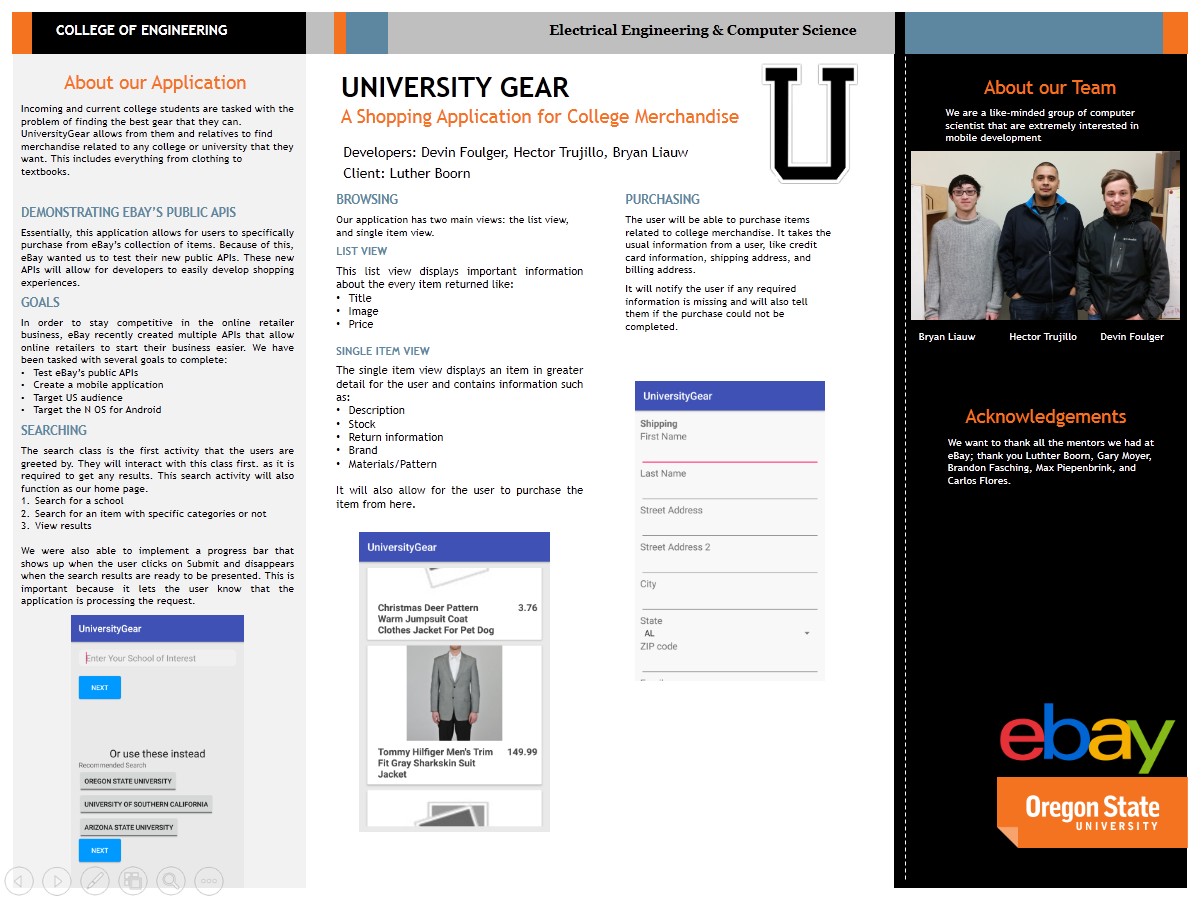
\includegraphics[angle=90,scale=.67]{expoPoster}
\end{figure}
\FloatBarrier

\section{Project Documentation}
UniversityGear was created to accomplish two major goals. The first being to help eBay
demonstrate how to use their APIs to individuals who want to create targeted eBay experiences.
The second goal is to create a targeted application that sells college or university related
merchandise. In order to do this, three major features were needed in the application:
searching, browsing, and purchasing.

\subsection{Searching}
The search feature of the application will allow the user to search for schools and specific
items. This works by first generating an OAuth V2 key from eBay. It then will send an HTTP
request to eBay's Browse API. This request will contain the user's specific search parameters
like price range, item name, school name, and categories. The result is an HTTP response with a
JSON object containing the items that it found. This information is then passed over to the
browsing feature of the application.

\subsection{Browsing}
There are two specific actions that are taken when browsing the item: browsing multiple results
at once and viewing a single result. First, a view with all the returned search results are
shown to the user. This is done by using the information from the returned search results. It
is then compiled into a RecyclerView where each item is clickable. These items all contain the
price, title, image, and ID of every item. Each ID is passed over to the single item view.
\newline

The single item view allows the user to view a single item in much greater detail. It will
contain the previously mentioned information as well as new information like the return and
shipping info, as well as the item brand, material, patterns, gender, and quantity. This is
done by taking the items ID and creating an HTTP request to eBay. It uses eBay's Browse API to
get the information of a single item. Like before, it will return a JSON object containing the
item's specific information. It will than parse this information and populate the view with the
information that it has received. If the user wants to purchase the item, they can click the
purchase button. This will pass the ID of the item to the purchase class.

\subsection{Purchasing}
The purchasing feature is rather straightforward. The ID is given from the single item view.
There are a lot of fields that the user must fill out. These included things like the shipping
information, credit card numbers, and billing information. If any of the information is
missing, it will return an error message and it won't let the user start the purchase. Once the
information is given, the purchase process can be started. This is done by using eBay's Order
API. It takes three separate HTTP requests to complete the purchasing process. The first is
initiating the checkout process. This needs to be done so that we can get a guest checkout ID.
This ID will be used in the other HTTP requests. The second HTTP request takes the guest
checkout ID and add the credit card information to the purchase. At this point, if the credit
card information does not work, it will return an error message to the user. The final HTTP
request will try to place the order. If the order is unsuccessful, it will return another error
message to the user. If the order was successful, it will notify the user that the order was
put through and give them an order ID.

\subsection{How to install and run}
In order to install the application on to a mobile device, it needs to specifically 
be an Android mobile device. It also needs to have the newest operating system 
to work properly. So, make sure that the device is on OS version 7. It should be 
noted that the application will run on tablet, but the user interface is not optimized 
for tablet use and it will not look correct. Once those requirements have been met, 
the APK will need to be downloaded from our GithHub repo here (https://github.com/FoulgerDevin/UniversityGear/releases).
Select the production APK if you want to purchase real items. If you want to 
specifically test the application, then use the sandbox APK. You will be able to 
purchase things without actually buying them. Once the APK has been installed, 
you can launch the application and use it. 

\begin{figure}[!h]
This is the flow that the user would take when using the application.
\centering
\caption{This is the user flow of the application.}
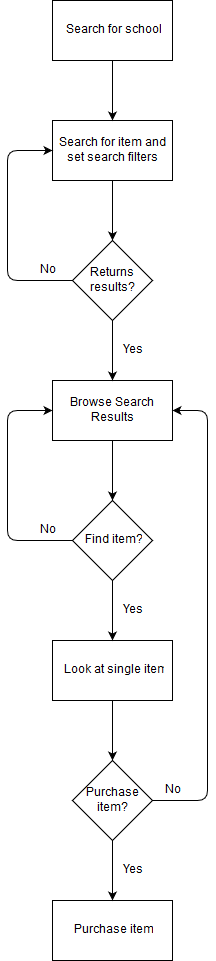
\includegraphics[scale=.67]{flowOfApp}
\end{figure}
\FloatBarrier

\section{Information Resources}
There were two main resources that the team used complete the application. The first method was
using common websites and eBay's documentation for their APIs. The second resource that the
group was able to use was eBay themselves. They were kind enough to give the group a set of
mentors that could be used to help if we were stuck on a specific process.

\subsection{Websites}
The common websites that were used were things like Stack Overflow, the Android Developer
website, and the eBay developer website. These resources greatly helped the team, because they
offered valuable coding examples and great documentation on specific APIs and how to use them.

\subsection{eBay Mentors}
The eBay mentors were of tremendous use as they were able to help the group with problems that
were undocumented. These problems pertained to eBay's new APIs, as they were new and many of
the problems we experienced were undocumented. Without their help, completing the application
in a timely manner would have been much harder. However, they helped us with many things like
looking at our code and showing us where we incorrectly used the APIs.

\section{Learning Experiences}
\subsection{Devin's Experiences}
\subsubsection{Technical}
Throughout the course of the project, there have been quite a few things that I 
have learned. When coming into this class, I had already done a minor amount of 
Android development. However, I learned how to better structure my design and 
code when developing. I also learned how to effectively use HTTP requests and 
how to use RESTful APIs. 

\subsubsection{Non-Technical}
Working with a team was an amazing experience. The biggest thing that I have 
learned is that communication will make things significantly easier. This includes 
communicating with our client throughout the term. I also learned that how to 
communicate professionally. Overall, I think that is the biggest key to success
in large groups. 

\subsubsection{Project Work}
I have found that project work is the most fun out any kind of work you can do.
Working with people is more fun. I also believe that the projects can be more 
in-depth and you can accomplish a lot more in a team. Working alone also isn't 
quite as fun, and I have found that team members are more likely to motivate 
you. I also learned that there is a methodological way to approaching a project.
A long amount of planning will significantly reduce the amount of coding you will 
have to do.

\subsubsection{Project Management}
I have learned that one of the best things that you can do is create a way to 
organize everything. For example, we used GitHub to share documents and to 
keep track of the changes that are constantly being made. Another thing in 
general is to have good communication. 

\subsubsection{Working in a Team}
I think that the best thing I have ever learned is that you have to be comfortable 
with the people you work with. By this, I mean you can't hate the people that you 
work with. You also need to learn how to take criticism or not to be offended when 
someone says your idea isn't good.

\subsubsection{What Would I Change}
If I were to change something, it would be to develop at a consistent pace 
throughout the whole term. I would develop in sprints, basically, and take a 
bit of time off from the next amount of work. I think the biggest reason that I 
wasn't able to do this is because I had other classes to worry about as well. I 
also probably would have started work earlier, like over winter term. Last, I 
think that we should have put more time into UI development.

\subsection{Bryan's Experiences}
\subsubsection{Technical}
Prior to this project, I've never worked extensively in a small group to create 
a mobile app. Personally, I feel my skills in mobile application development 
improved immensely. It feels different using Java to create a mobile 
application than to create a regular application. I also worked with HTTP 
RESTful requests. While I have worked on other third party API, learning how 
to send requests through HTTP is new for me. It is also more efficient in terms 
of programming it.

\subsubsection{Non-Technical}
Since this project is time-consuming, I need to be able to balance classes, 
personal commitments, etc. This requires an effective time management, 
which I believe a skill I learned during the project. 

\subsubsection{Project Work}
Doing things in time is important in doing projects as a group. Since every 
parts of this project is dependent of each other in order to run, we need 
things to be in time. 

\subsubsection{Project Management}
I learned how to plan and run that plan with my group members. 

\subsubsection{Working in a Team}
This is the first time I worked extensively with a group for a long period of 
time on a project. I learned how communication is really vital in working in a 
group. Dividing the work so that everything can be done in time is also really 
crucial.

\subsubsection{What Would I Change}
If I were to do something differently, I would start earlier than I did. We 
started our work during the Winter term. I believe we could have a much smoother 
run if we had started during the break. Furthermore, we seemed to go off during 
the breaks. While it is justified, I believe our testing and development could be 
done earlier, thus leaving more room for us to improve. I would also focus more 
on UI development, because I believe that our UI is under-developed. If we 
had more time, we could have showcased a better UI during expo.  Another thing 
I would change is I would pay more attention to details in the documentation. We 
were stumped by minor things that was only rectified after we re-read the 
documentation in details. If we had done that earlier, we could save time 
debugging.

\subsection{Hector's Experiences}
\subsubsection{Technical}
I learned plenty of technical information during this project. I had never 
developed a mobile application of any kind. I got a good understanding of 
the development process for Android Development and it's core features.
 I learned about starting new activities and passing data from one activity 
 to the other. I also learned about displaying data using different android 
 components such as RecyclerView and ListView. I also, learned how to 
 handle user clicks and scrolling through data. Also, by looking at the other 
 features implemented by the rest of the team I was able to get a feel for 
 using HTTP RESTful third party API calls.

\subsubsection{Non-Technical}
Biggest non-technical information that I learned is that communication is 
critical when working with a large team. Frequent communication will eliminate 
confusions and will keep the entire team up to date about what is going on 
with the project. Also, I got a good understanding on how the communication 
method and format can vary depending on the issue that is being 
communicated. A simple question can be discussed through email, while a 
critical issue will likely require a face-to-face meeting.

\subsubsection{Project Work}
It;s very important to be accountable for the items that you are responsible 
for. The rest of the project is going to be dependent on those pieces. It's also 
useful to set development guidelines from the get go. This will help whenever 
someone needs to work on pieces of code that they did not implement. 

\subsubsection{Project Management}
I learned that it is important to make good estimates when trying to come up 
with a project schedule. There were times, when I had to work extra hard to 
meet our estimated schedule and keep the project on track. I also learned that 
it's important to keep constant communication with the rest of the project team.

\subsubsection{Working in a Team}
It's difficult to work in teams when each member has many different things 
going on at the same time. Trying to schedule team meetings with everyone 
is nearly impossible. I also learned that using your team members as resources 
is very beneficial and will save you plenty of time over trying to figure it out 
on your own.

\subsubsection{What Would I Change}
After meeting with the client, we got a better understanding for the project. 
At this point, I realized that the project was not what I was expecting. This 
was discouraging and brought my level of interest in the project down. The 
first thing that I would do differently is to really vet the projects that seem 
interesting to me. This will help me avoid getting into projects that aren't as 
interesting as they first appear. As far as actually working on the project, 
things that I would do differently include making a firm schedule and keeping 
to it. For the duration of the course, my scheduling consisted of I have to 
get X done by this date. Failing to set hard dates to work on X left me 
procrastinating and stressing out last minute to get items done on time. 
Another thing that I would do differently would be to not settle for the minimum 
requirements. After some of the minimum requirements were made, 
refinements could have been made to the code and the implementation to 
improve functionality and user experience. 

\section{Appendix I Listings}

\subsection{Essential Code Listings}
There is one bit of code that was essential to completing the project. This was 
building the HTTP requests used to complete searching and purchasing. They 
are specifically used to use eBay's RESTful APIs. Here is an example of what a 
request would look like for initiating the guest purchase session. The others are very similar, 
but have differences in parameters, depending on which API call is used. 

\begin{lstlisting}
        /*
         * This method is used to initiate the guest checkout session
         * Inputs: User info JSON
         * Returns: checkoutSessionId
         */
        private String initiateOrder(JSONObject userInfo) {
            URL purchaseUrl = null;
            HttpURLConnection apiConnection = null;
            InputStream sessionStream;
            JSONObject purchaseInitiateJSON;
            String streamResult = null;

            //set the URL to be used in starting the purchase session
            String purchaseUrlString = getString(R.string.purchaseInitiateUrl);

            try {
                purchaseUrl = new URL(purchaseUrlString);
            } catch(MalformedURLException e) {
                e.printStackTrace();
                Log.e("PURCHASE URL", "URL Failed");
            }

            //Open the connection using the purchase url
            try {
                apiConnection = (HttpURLConnection)purchaseUrl.openConnection();
                apiConnection.setDoInput(true);
                apiConnection.setDoOutput(true);
            } catch(IOException e) {
                e.printStackTrace();
                Log.e("CONNECTION","Failed to connect");
            }

            //Set the correct header information

            SharedPreferences sharedPreferences = getSharedPreferences(
            			"Authentication", Context.MODE_PRIVATE);
            Log.i("OAuth Token INITIATE", sharedPreferences.getString("oAuthToken2", ""));
            apiConnection.setRequestProperty("Authorization", "Bearer " + 
            			sharedPreferences.getString("oAuthToken2",""));
            apiConnection.setRequestProperty("Accept", "application/json");
            apiConnection.setRequestProperty(
            			"Content-Type", "application/json; charset=UTF-8");

            //Set the correct request method
            try {
                apiConnection.setRequestMethod("POST");
                OutputStream os = apiConnection.getOutputStream();
                os.write(userInfo.toString().getBytes("UTF-8"));
                os.close();
            } catch(ProtocolException e) {
                e.printStackTrace();
                Log.e("REQUEST METHOD", "Failed to set request method to POST");
            } catch(IOException e) {
                Log.e("OUTPUT STREAM WRITER", "Could not write to stream");
            }

            Log.e("API CONNECTION", "Connection: " + apiConnection);

            //get the response code
            int responseCode = 0;
            try {
                responseCode = apiConnection.getResponseCode();
                Log.i("RESPONSE CODE", "Response code: " + responseCode);
            } catch(IOException e) {
                e.printStackTrace();
                Log.e("RESPONSE CODE", "Response code: " + responseCode);
            }

            //Open the input stream
            if (responseCode == 200) {
                try {
                    sessionStream = apiConnection.getInputStream();
                    BufferedReader r = new BufferedReader
                    			(new InputStreamReader(sessionStream));
                    StringBuilder total = new StringBuilder();
                    String line;
                    while ((line = r.readLine()) != null) {
                        total.append(line).append('\n');
                    }

                    streamResult = total.toString();
                    //streamResult  = getStringFromInputStream(sessionStream);
                } catch (IOException e) {
                    e.printStackTrace();
                    Log.e("SESSION STREAM", "Could not get a session stream string");
                }

                //Create a JSON object from the returned streamResult and get
                //the checkoutSessionId
                try {
                    purchaseInitiateJSON = new JSONObject(streamResult);
                    if (streamResult.contains("checkoutSessionId")) {
                        checkoutSessionId = purchaseInitiateJSON.getString(
                        			"checkoutSessionId");
                    }
                } catch (JSONException e) {
                    Log.e("JSON CREATION", "Failed to create a JSON object");
                }

                if (checkoutSessionId != null) {
                    Log.i("CHECKOUT ID", "" + checkoutSessionId);
                } else {
                    Log.i("CHECKOUT ID", "is null");
                }

                Log.i("INITIATE","SUCCESS");
            } else {
                Log.e("INITIATE","FAILED");
            }

            return checkoutSessionId;
        }
\end{lstlisting}

\section{Appendix II Photos}

\begin{figure}[!h]
This is an image of the home screen and it is the first thing the user sees. 
\centering
\caption{Home Screen}

\includegraphics[scale=.11]{homeScreen}
\end{figure}
\FloatBarrier

\begin{figure}[!h]
This is the search screen, which comes after when the user selects a school. It 
will allow them to filter search results.
\centering
\caption{Search Screen}
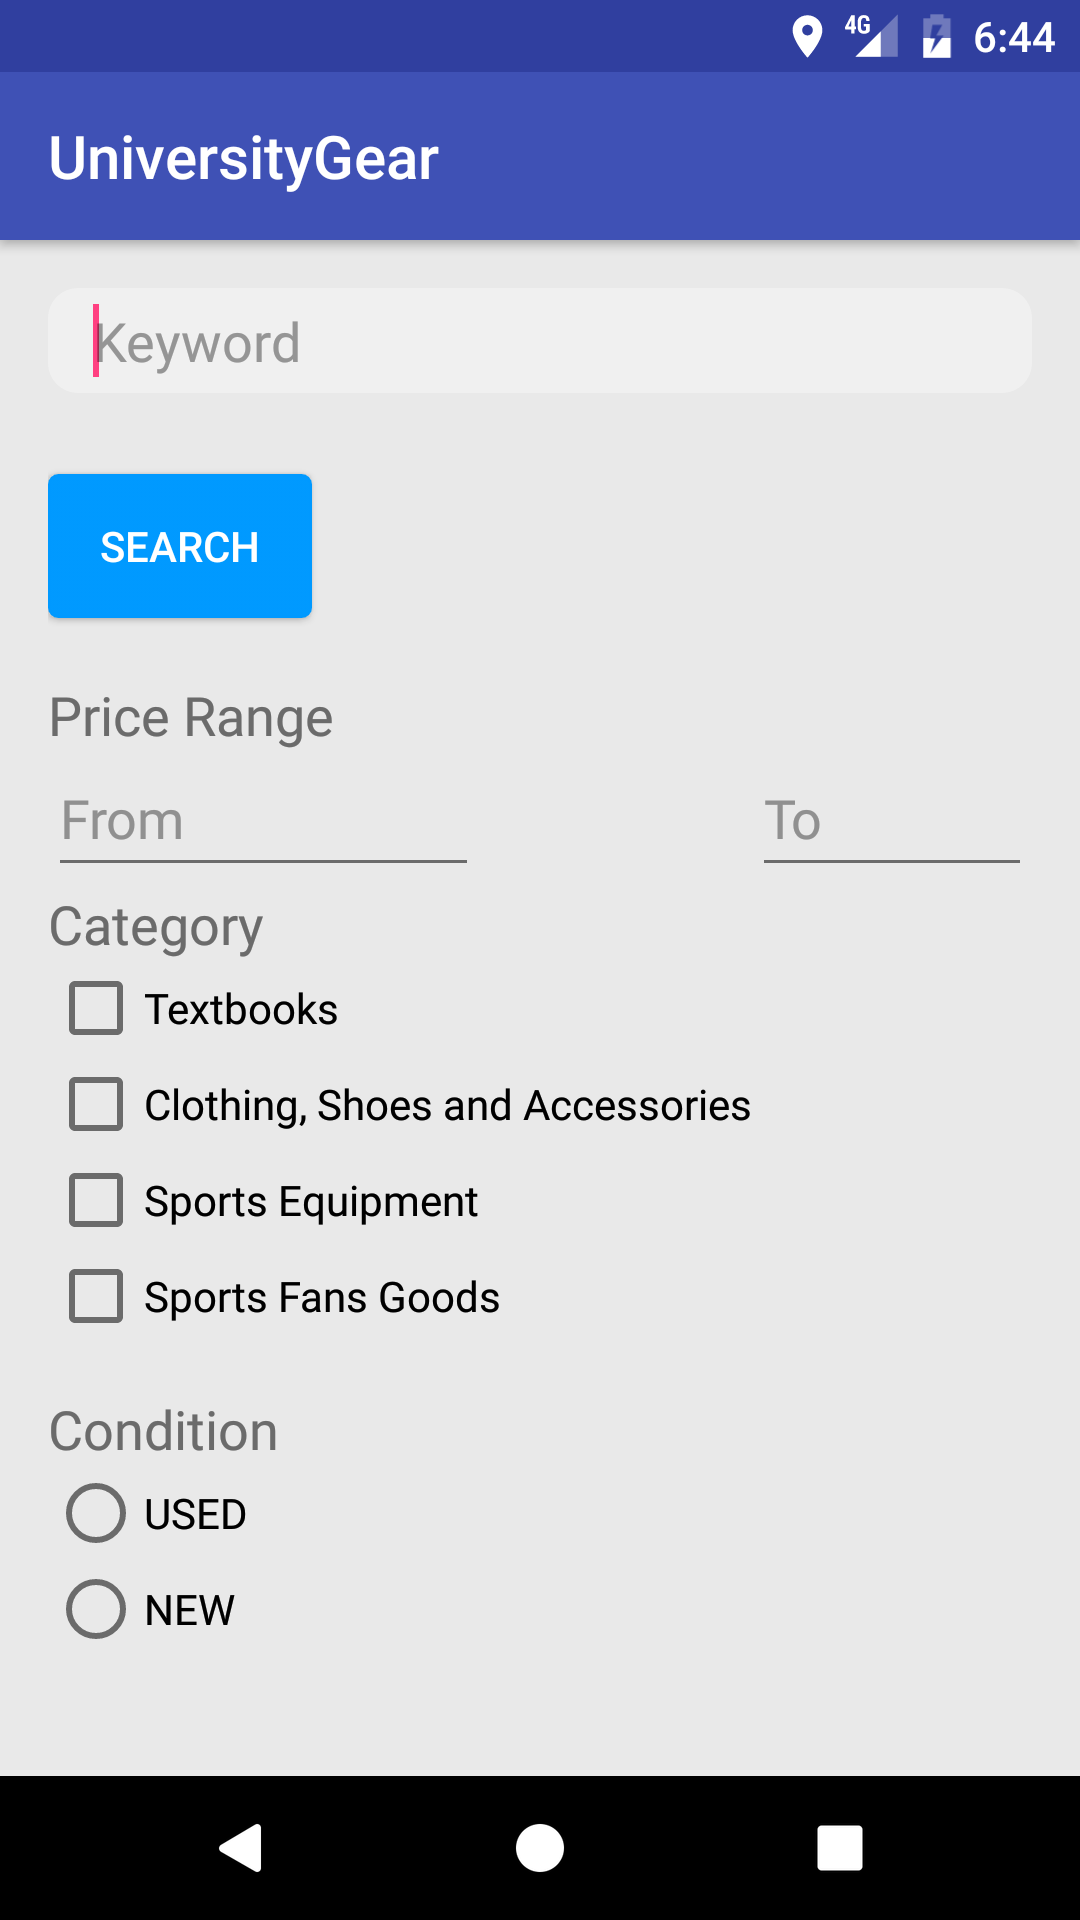
\includegraphics[scale=.15]{searchScreen}
\end{figure}
\FloatBarrier

\begin{figure}[!h]
Here is what it looks like when results are returned. 
\centering
\caption{Search Results}
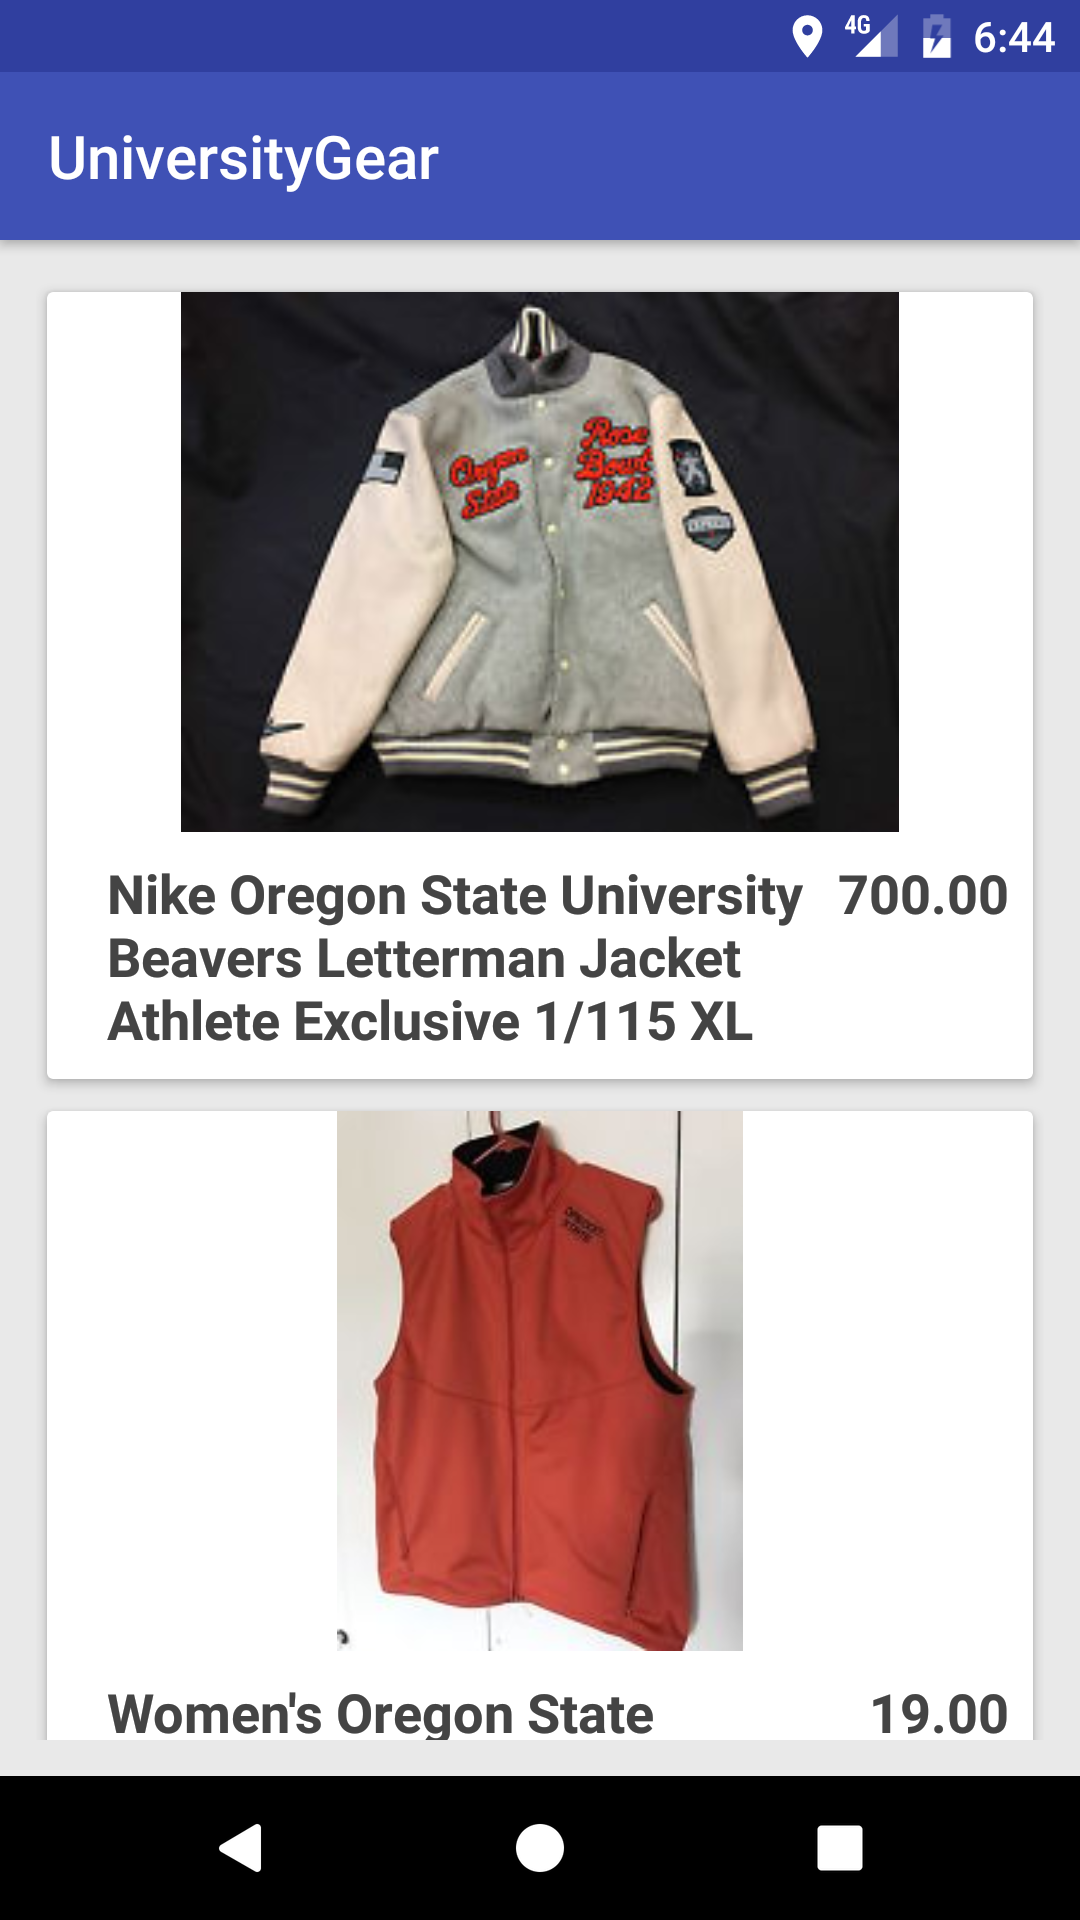
\includegraphics[scale=.15]{results}
\end{figure}
\FloatBarrier

\begin{figure}[!h]
This is what it looks like when you are viewing a single item. It gives the user 
a wide variety of information on that item. 
\centering
\caption{Viewing an item (top half)}
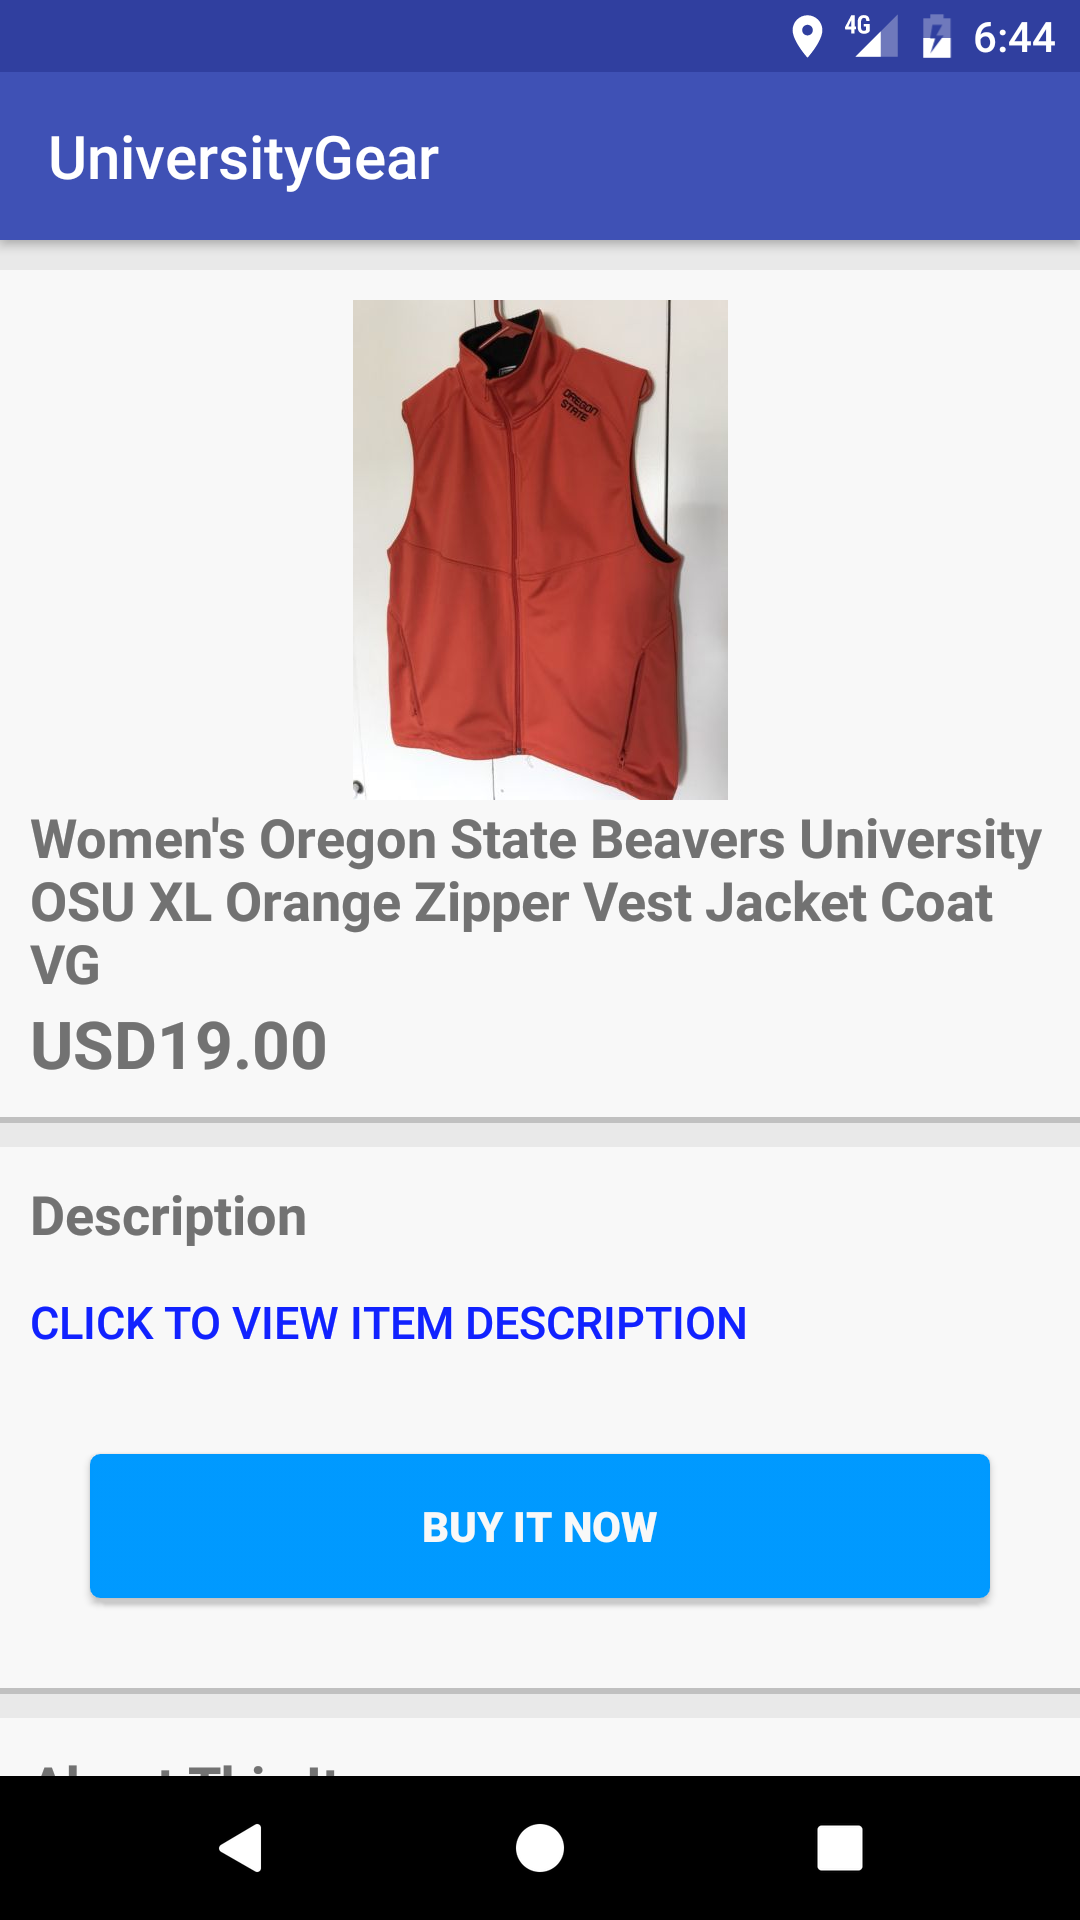
\includegraphics[scale=.13]{singleItem1}
\end{figure}
\FloatBarrier

\begin{figure}[!h]
This is what kind of information you can get for a single item.
\centering
\caption{Viewing an item (bottom half)}
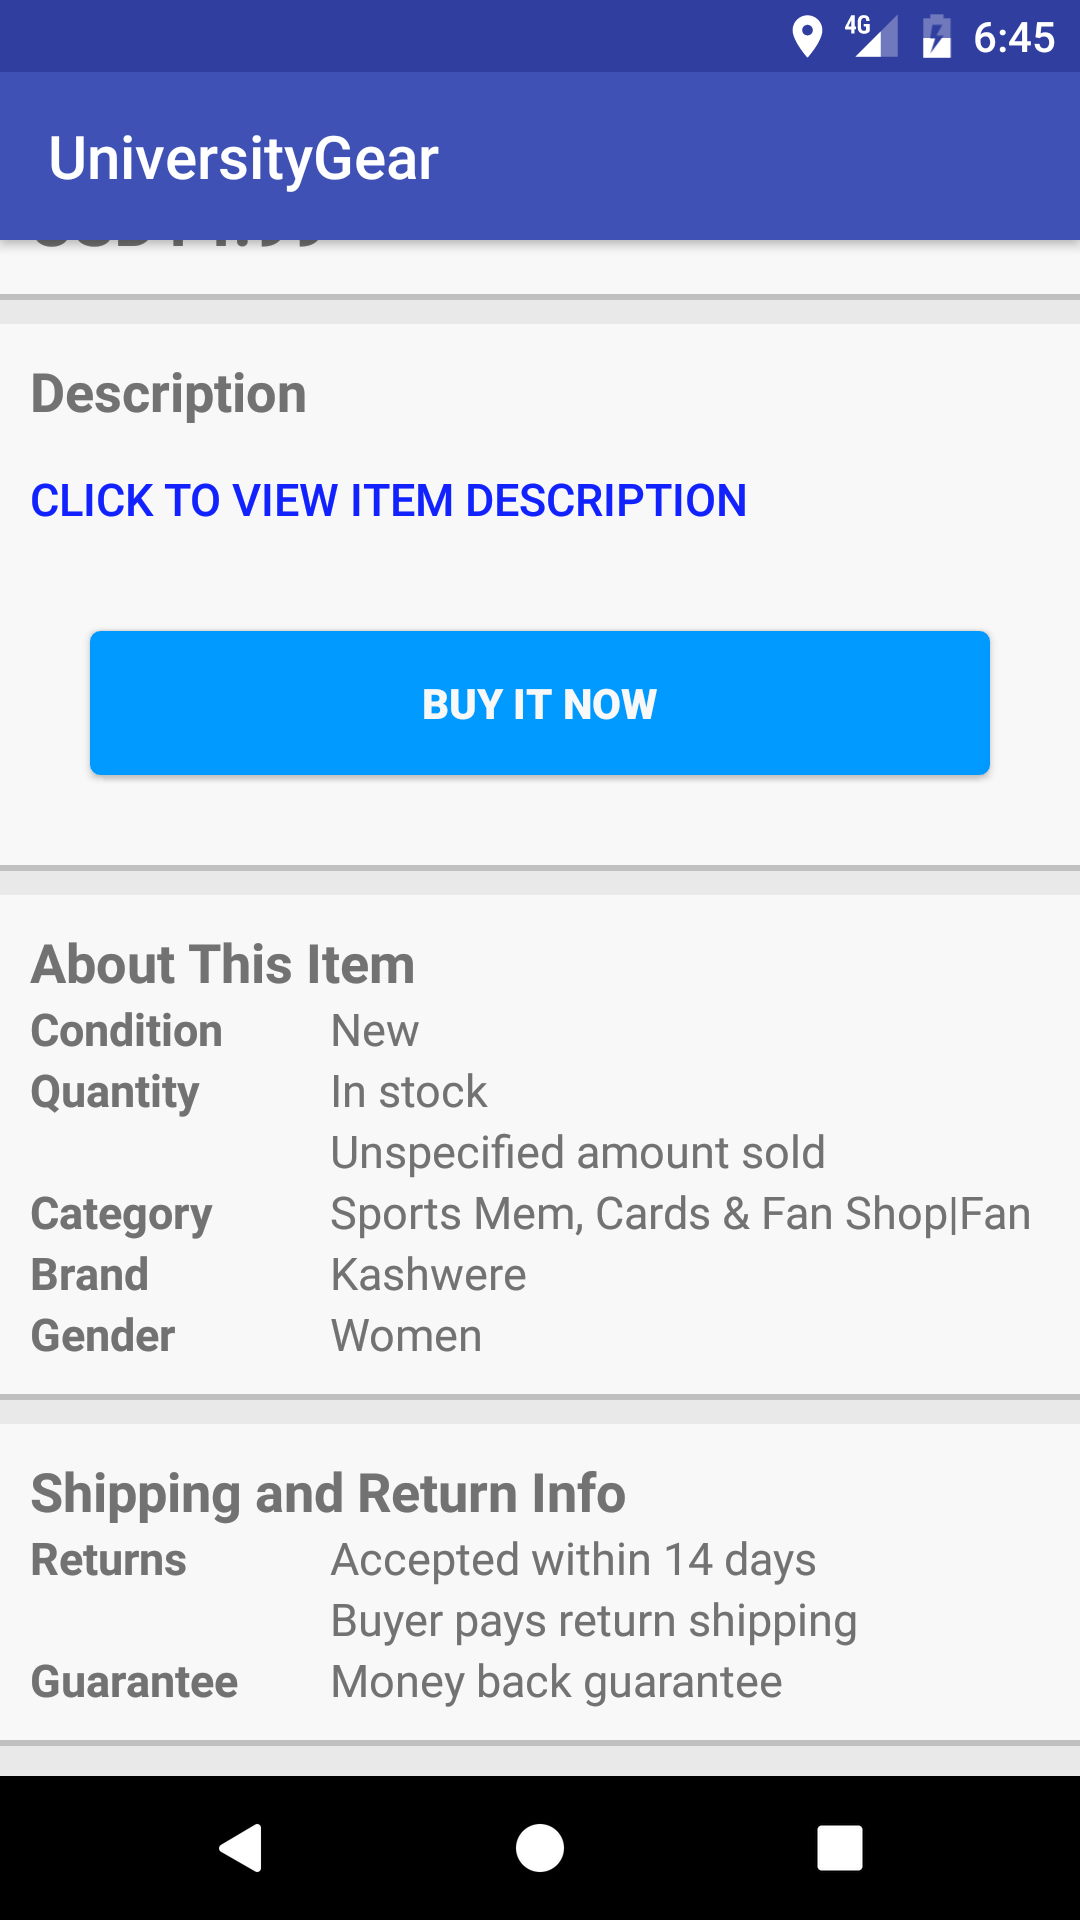
\includegraphics[scale=.15]{singleItem2}
\end{figure}
\FloatBarrier

\begin{figure}[!h]
This is the description of a single item. It is in a webview, because some 
sellers have custom store pages.
\centering
\caption{Item Description}
\includegraphics[scale=.15]{webview}
\end{figure}
\FloatBarrier

\begin{figure}[!h]
The purchasing screen is rather forward and asks for all of the users information.
\centering
\caption{Purchasing Screen}
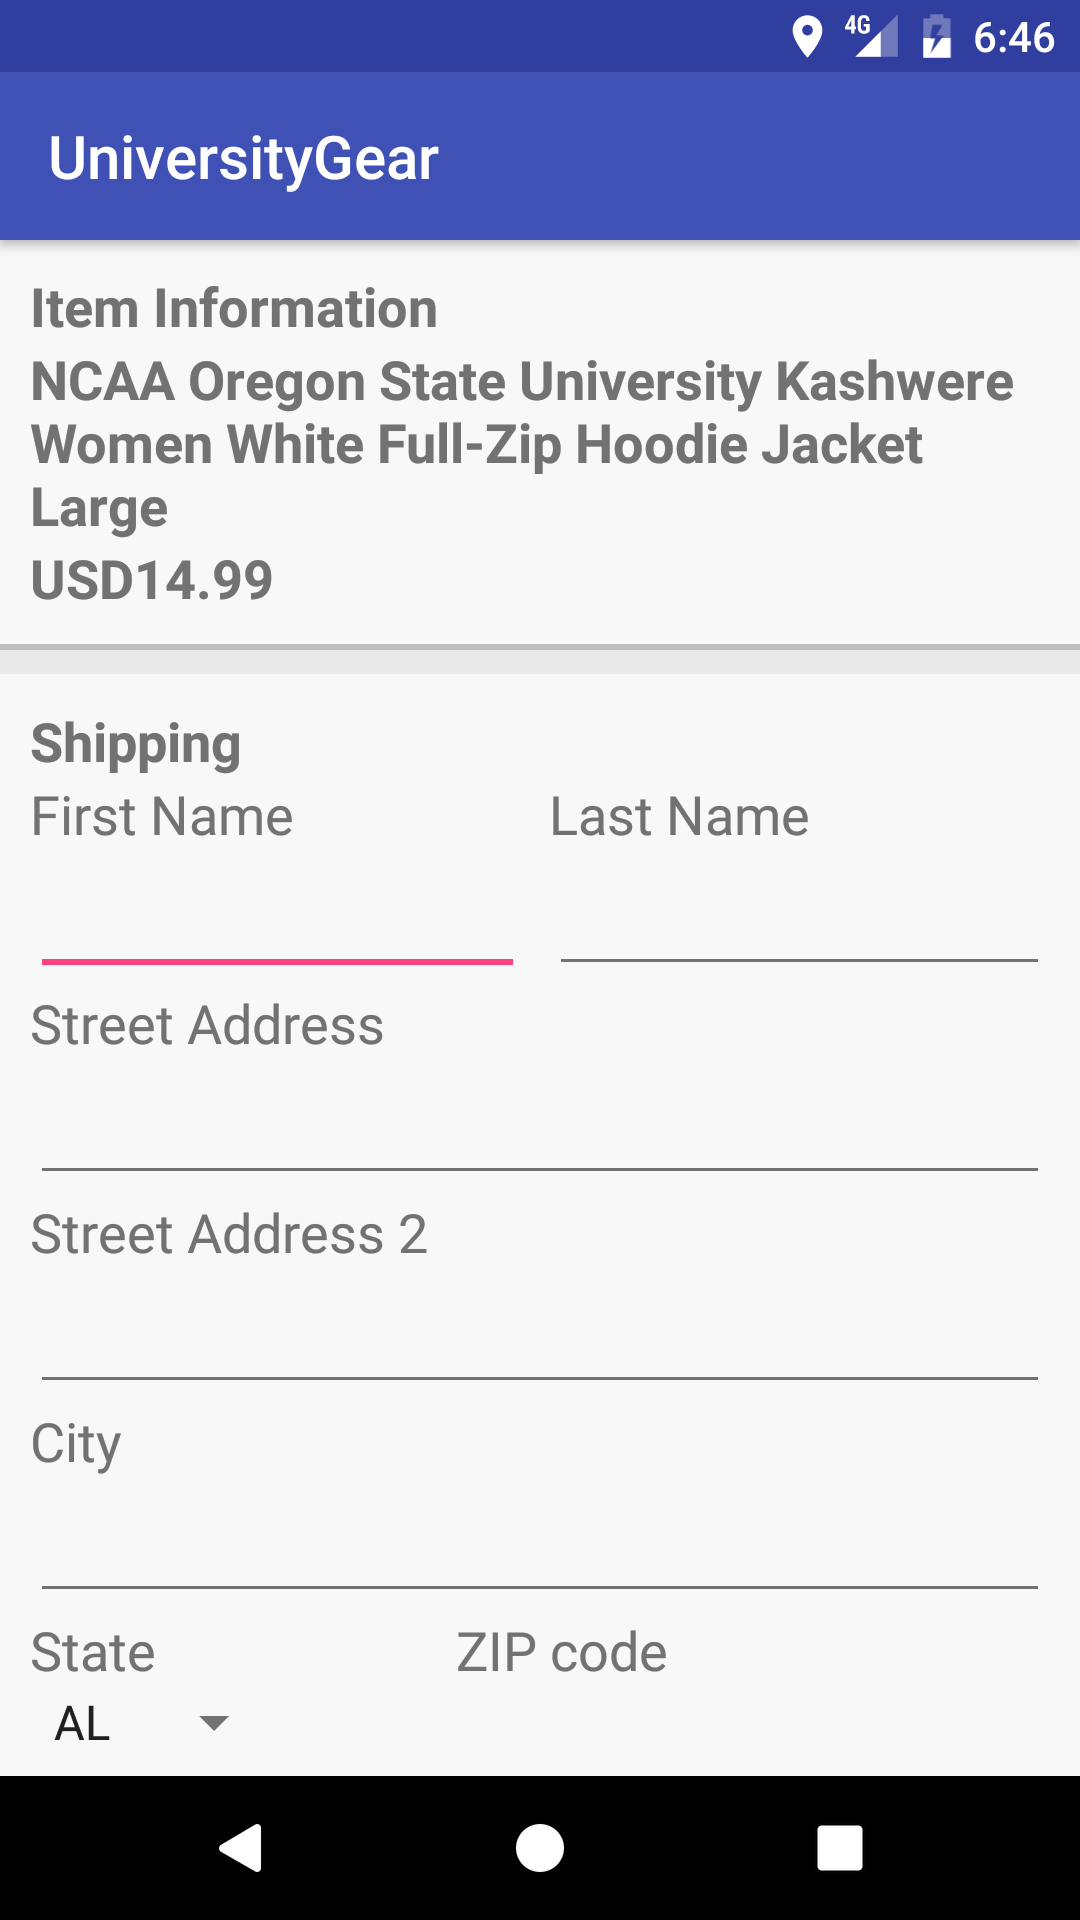
\includegraphics[scale=.13]{purchase}
\end{figure}
\FloatBarrier

\begin{figure}[!h]
This is what happens when there is no internet connection.
\centering
\caption{No Internet Error Message}
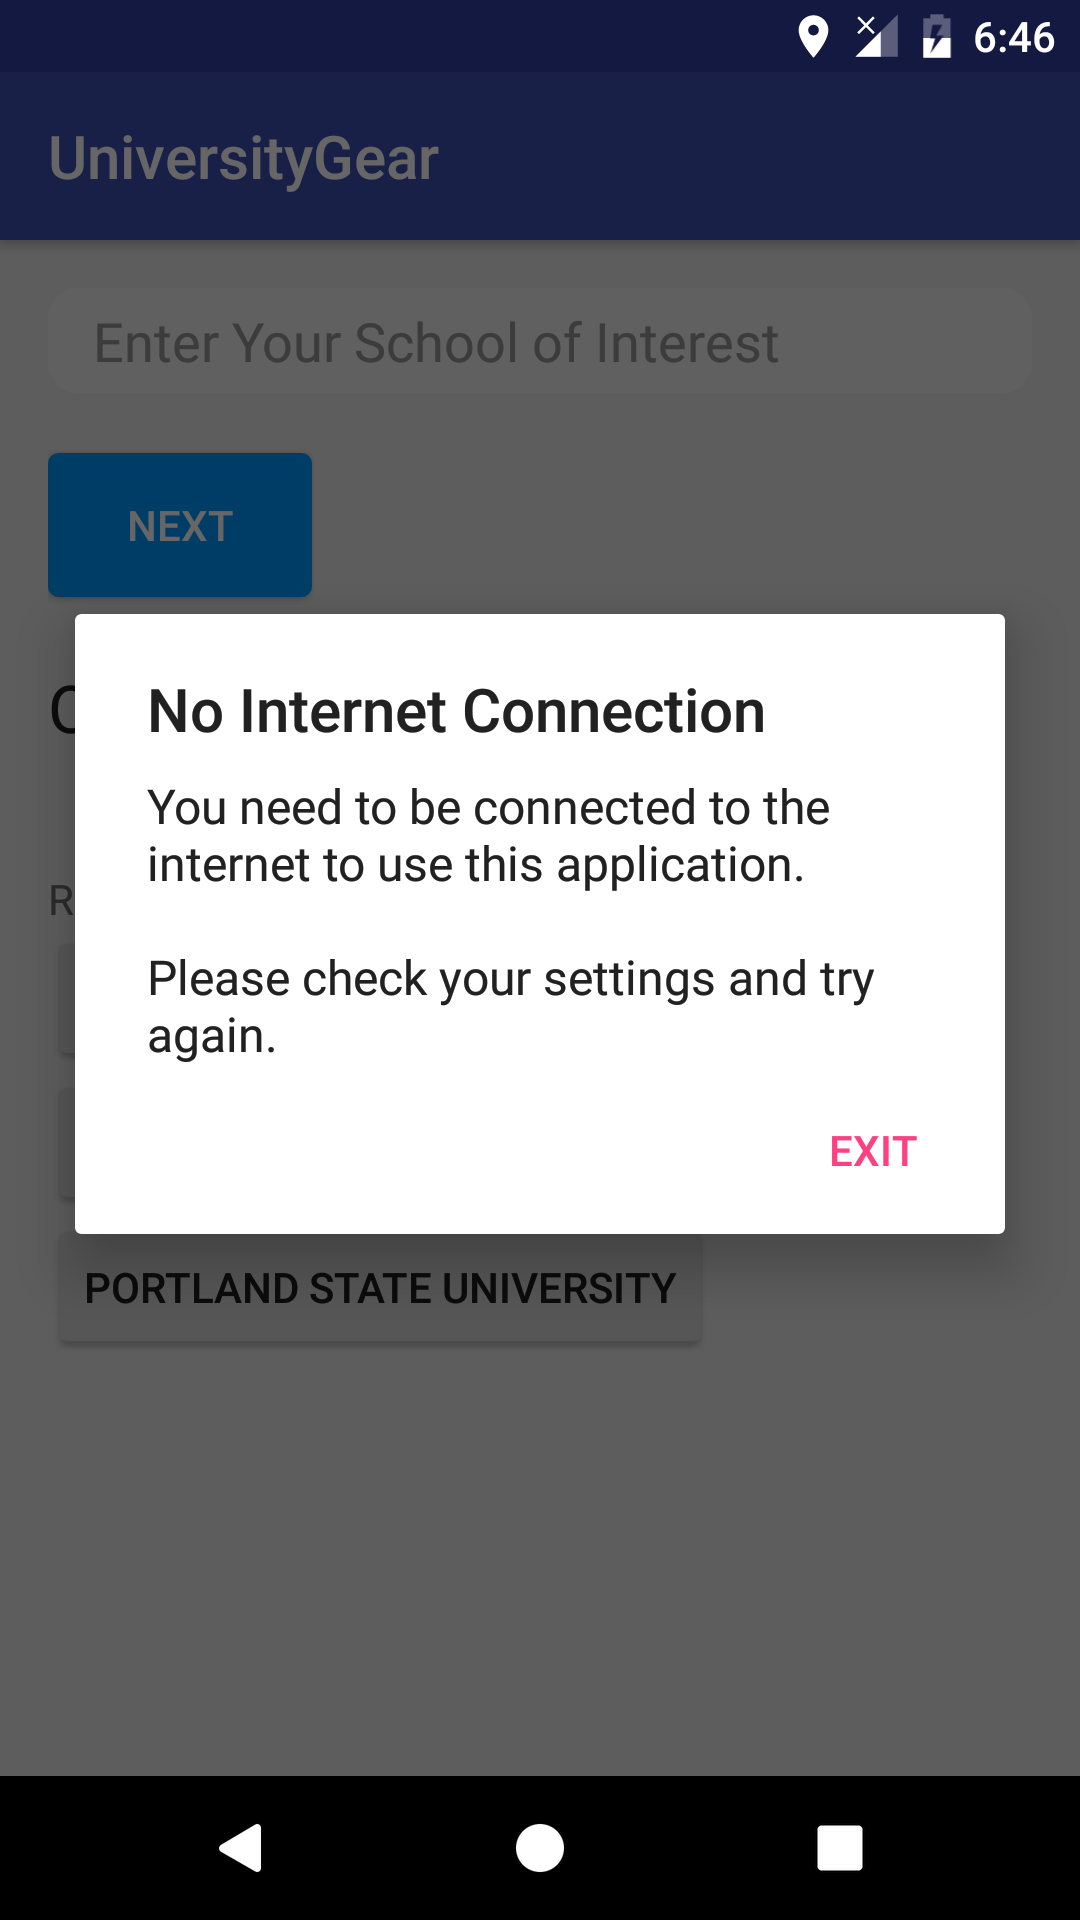
\includegraphics[scale=.15]{noInternetError}
\end{figure}
\FloatBarrier

\begin{figure}[!h]
This is what happens when no search results are found. 
\centering
\caption{No Search Results Message}
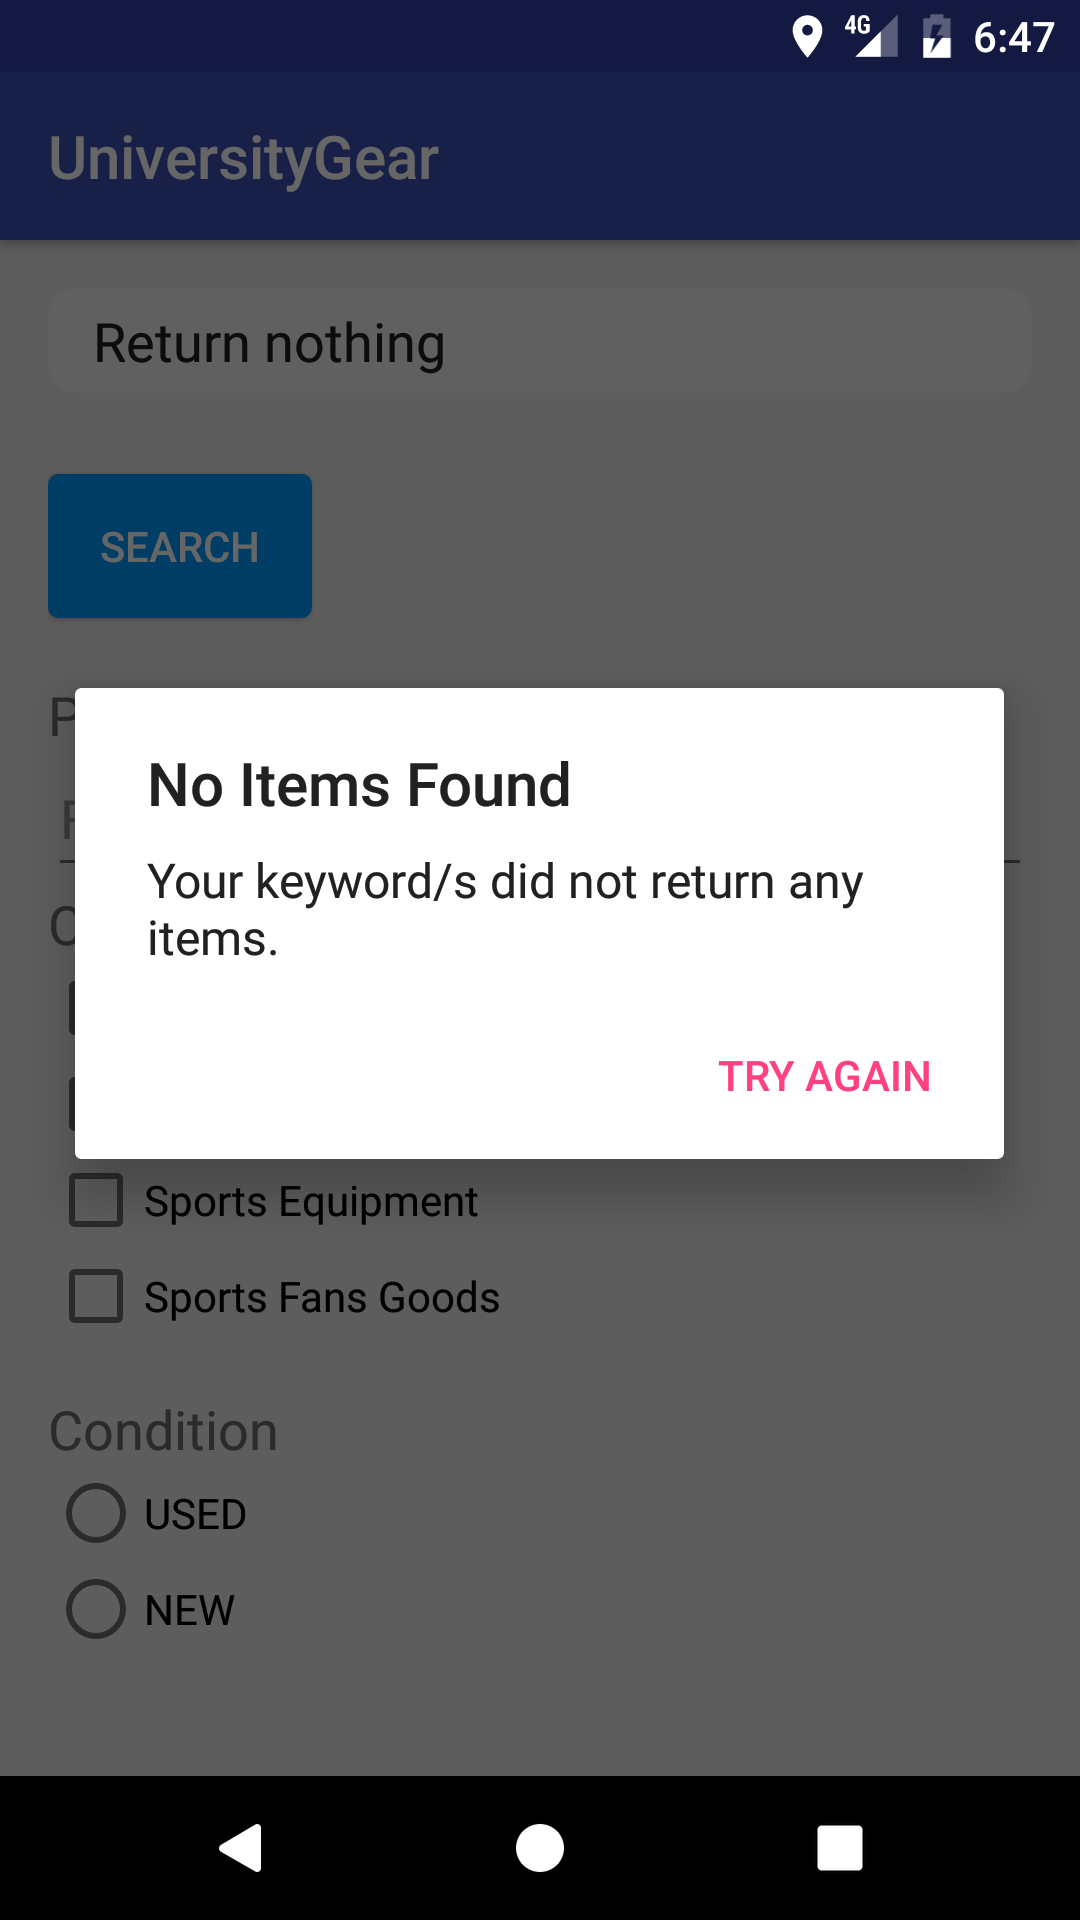
\includegraphics[scale=.15]{noSearchResults}
\end{figure}
\FloatBarrier

\end{document}
